
%% Beginning of file 'sample63.tex'
%%
%% Modified 2019 June
%%
%% This is a sample manuscript marked up using the
%% AASTeX v6.3 LaTeX 2e macros.
%%
%% AASTeX is now based on Alexey Vikhlinin's emulateapj.cls 
%% (Copyright 2000-2015).  See the classfile for details.

%% AASTeX requires revtex4-1.cls (http://publish.aps.org/revtex4/) and
%% other external packages (latexsym, graphicx, amssymb, longtable, and epsf).
%% All of these external packages should already be present in the modern TeX 
%% distributions.  If not they can also be obtained at www.ctan.org.

%% The first piece of markup in an AASTeX v6.x document is the \documentclass
%% command. LaTeX will ignore any data that comes before this command. The 
%% documentclass can take an optional argument to modify the output style.
%% The command below calls the preprint style which will produce a tightly 
%% typeset, one-column, single-spaced document.  It is the default and thus
%% does not need to be explicitly stated.
%%
%%
%% using aastex version 6.3
\documentclass[twocolumn]{./aastex63}

\usepackage{amsmath}
\usepackage{empheq}
\usepackage{mathrsfs}
\usepackage{textcomp}
\usepackage{enumitem}   
\usepackage{gensymb}
\usepackage{hyperref}
\usepackage{graphicx}
\usepackage[caption=false]{subfig}
\usepackage{multirow}
\usepackage{longtable}
\hypersetup{colorlinks, linkcolor={blue}, citecolor={blue}, urlcolor={blue}} 
%% The default is a single spaced, 10 point font, single spaced article.
%% There are 5 other style options available via an optional argument. They
%% can be invoked like this:
%%
%% \documentclass[arguments]{aastex63}
%% 
%% where the layout options are:
%%
%%  twocolumn   : two text columns, 10 point font, single spaced article.
%%                This is the most compact and represent the final published
%%                derived PDF copy of the accepted manuscript from the publisher
%%  manuscript  : one text column, 12 point font, double spaced article.
%%  preprint    : one text column, 12 point font, single spaced article.  
%%  preprint2   : two text columns, 12 point font, single spaced article.
%%  modern      : a stylish, single text column, 12 point font, article with
%% 		  wider left and right margins. This uses the Daniel
%% 		  Foreman-Mackey and David Hogg design.
%%  RNAAS       : Preferred style for Research Notes which are by design 
%%                lacking an abstract and brief. DO NOT use \begin{abstract}
%%                and \end{abstract} with this style.
%%
%% Note that you can submit to the AAS Journals in any of these 6 styles.
%%
%% There are other optional arguments one can invoke to allow other stylistic
%% actions. The available options are:
%%
%%   astrosymb    : Loads Astrosymb font and define \astrocommands. 
%%   tighten      : Makes baselineskip slightly smaller, only works with 
%%                  the twocolumn substyle.
%%   times        : uses times font instead of the default
%%   linenumbers  : turn on lineno package.
%%   trackchanges : required to see the revision mark up and print its output
%%   longauthor   : Do not use the more compressed footnote style (default) for 
%%                  the author/collaboration/affiliations. Instead print all
%%                  affiliation information after each name. Creates a much 
%%                  longer author list but may be desirable for short 
%%                  author papers.
%% twocolappendix : make 2 column appendix.
%%   anonymous    : Do not show the authors, affiliations and acknowledgments 
%%                  for dual anonymous review.
%%
%% these can be used in any combination, e.g.
%%
%% \documentclass[twocolumn,linenumbers,trackchanges]{aastex63}
%%
%% AASTeX v6.* now includes \hyperref support. While we have built in specific
%% defaults into the classfile you can manually override them with the
%% \hypersetup command. For example,
%%
%% \hypersetup{linkcolor=red,citecolor=green,filecolor=cyan,urlcolor=magenta}
%%
%% will change the color of the internal links to red, the links to the
%% bibliography to green, the file links to cyan, and the external links to
%% magenta. Additional information on \hyperref options can be found here:
%% https://www.tug.org/applications/hyperref/manual.html#x1-40003
%%
%% Note that in v6.3 "bookmarks" has been changed to "true" in hyperref
%% to improve the accessibility of the compiled pdf file.
%%
%% If you want to create your own macros, you can do so
%% using \newcommand. Your macros should appear before
%% the \begin{document} command.
%%
\newcommand{\vdag}{(v)^\dagger}
\newcommand\aastex{AAS\TeX}
\newcommand\latex{La\TeX}

%%%%%%%%%%%%%%%%%%%%%%%%%%%%%%%%%%%%%%%%%%%%%%%%%%%%%%%%%%%%%%%%%%%%%%%%%%%%%%%%
%%
%% The following section defines new commands for comments from co-authors
%%
\definecolor{DarkOrange}{RGB}{204, 85, 0}
\definecolor{LincolnGreen}{RGB}{17, 102, 0}
\def\ion#1#2{#1$\;${\footnotesize\rm{#2}}\relax}

\newcommand{\yy}[1]{{\color{red} yy: {#1}}}
\newcommand{\aam}[1]{{\color{DarkOrange} aam: {#1}}}
\newcommand{\todo}[1]{{\color{magenta} to-do: {#1}}}

\newcommand{\rztf}{$r_\mathrm{ZTF}$}
\newcommand{\gztf}{$g_\mathrm{ZTF}$}
\newcommand{\tfl}{$t_\mathrm{fl}$}
\newcommand{\trise}{$t_\mathrm{rise}$}
\newcommand{\tbmax}{$t_{B,\mathrm{max}}$}
%%
%%%%%%%%%%%%%%%%%%%%%%%%%%%%%%%%%%%%%%%%%%%%%%%%%%%%%%%%%%%%%%%%%%%%%%%%%%%%%%%%

%% Reintroduced the \received and \accepted commands from AASTeX v5.2
\received{\today}
% \revised{January 10, 2019}
% \accepted{\today}
%% Command to document which AAS Journal the manuscript was submitted to.
%% Adds "Submitted to " the argument.
\submitjournal{ApJ}

%% For manuscript that include authors in collaborations, AASTeX v6.3
%% builds on the \collaboration command to allow greater freedom to 
%% keep the traditional author+affiliation information but only show
%% subsets. The \collaboration command now must appear AFTER the group
%% of authors in the collaboration and it takes TWO arguments. The last
%% is still the collaboration identifier. The text given in this
%% argument is what will be shown in the manuscript. The first argument
%% is the number of author above the \collaboration command to show with
%% the collaboration text. If there are authors that are not part of any
%% collaboration the \nocollaboration command is used. This command takes
%% one argument which is also the number of authors above to show. A
%% dashed line is shown to indicate no collaboration. This example manuscript
%% shows how these commands work to display specific set of authors 
%% on the front page.
%%
%% For manuscript without any need to use \collaboration the 
%% \AuthorCollaborationLimit command from v6.2 can still be used to 
%% show a subset of authors.
%
%\AuthorCollaborationLimit=2
%
%% will only show Schwarz & Muench on the front page of the manuscript
%% (assuming the \collaboration and \nocollaboration commands are
%% commented out).
%%
%% Note that all of the author will be shown in the published article.
%% This feature is meant to be used prior to acceptance to make the
%% front end of a long author article more manageable. Please do not use
%% this functionality for manuscripts with less than 20 authors. Conversely,
%% please do use this when the number of authors exceeds 40.
%%
%% Use \allauthors at the manuscript end to show the full author list.
%% This command should only be used with \AuthorCollaborationLimit is used.

%% The following command can be used to set the latex table counters.  It
%% is needed in this document because it uses a mix of latex tabular and
%% AASTeX deluxetables.  In general it should not be needed.
%\setcounter{table}{1}

%%%%%%%%%%%%%%%%%%%%%%%%%%%%%%%%%%%%%%%%%%%%%%%%%%%%%%%%%%%%%%%%%%%%%%%%%%%%%%%%
%%
%% The following section outlines numerous optional output that
%% can be displayed in the front matter or as running meta-data.
%%
%% If you wish, you may supply running head information, although
%% this information may be modified by the editorial offices.
\shorttitle{The Rise of ZTF SNe Ia}
\shortauthors{Miller et al.}
%%
%% You can add a light gray and diagonal water-mark to the first page 
%% with this command:
\watermark{DRAFT}
%% where "text", e.g. DRAFT, is the text to appear.  If the text is 
%% long you can control the water-mark size with:
%% \setwatermarkfontsize{dimension}
%% where dimension is any recognized LaTeX dimension, e.g. pt, in, etc.
%%
%%%%%%%%%%%%%%%%%%%%%%%%%%%%%%%%%%%%%%%%%%%%%%%%%%%%%%%%%%%%%%%%%%%%%%%%%%%%%%%%

%% This is the end of the preamble.  Indicate the beginning of the
%% manuscript itself with \begin{document}.

\begin{document}

\title{ZTF Early Observations of Type Ia  Supernovae II: \\ First Light, the Initial Rise, and Time to Reach Maximum Brightness}

%% LaTeX will automatically break titles if they run longer than
%% one line. However, you may use \\ to force a line break if
%% you desire. In v6.3 you can include a footnote in the title.

%% A significant change from earlier AASTEX versions is in the structure for 
%% calling author and affiliations. The change was necessary to implement 
%% auto-indexing of affiliations which prior was a manual process that could 
%% easily be tedious in large author manuscripts.
%%
%% The \author command is the same as before except it now takes an optional
%% argument which is the 16 digit ORCID. The syntax is:
%% \author[xxxx-xxxx-xxxx-xxxx]{Author Name}
%%
%% This will hyperlink the author name to the author's ORCID page. Note that
%% during compilation, LaTeX will do some limited checking of the format of
%% the ID to make sure it is valid. If the "orcid-ID.pdf" image file is 
%% present or in the LaTeX pathway, the OrcID icon will appear next to
%% the authors name.
%%
%% Use \affiliation for affiliation information. The old \affil is now aliased
%% to \affiliation. AASTeX v6.3 will automatically index these in the header.
%% When a duplicate is found its index will be the same as its previous entry.
%%
%% Note that \altaffilmark and \altaffiltext have been removed and thus 
%% can not be used to document secondary affiliations. If they are used latex
%% will issue a specific error message and quit. Please use multiple 
%% \affiliation calls for to document more than one affiliation.
%%
%% The new \altaffiliation can be used to indicate some secondary information
%% such as fellowships. This command produces a non-numeric footnote that is
%% set away from the numeric \affiliation footnotes.  NOTE that if an
%% \altaffiliation command is used it must come BEFORE the \affiliation call,
%% right after the \author command, in order to place the footnotes in
%% the proper location.
%%
%% Use \email to set provide email addresses. Each \email will appear on its
%% own line so you can put multiple email address in one \email call. A new
%% \correspondingauthor command is available in V6.3 to identify the
%% corresponding author of the manuscript. It is the author's responsibility
%% to make sure this name is also in the author list.
%%
%% While authors can be grouped inside the same \author and \affiliation
%% commands it is better to have a single author for each. This allows for
%% one to exploit all the new benefits and should make book-keeping easier.
%%
%% If done correctly the peer review system will be able to
%% automatically put the author and affiliation information from the manuscript
%% and save the corresponding author the trouble of entering it by hand.

\correspondingauthor{Adam A. Miller}
\email{amiller@northwestern.edu}

\author[0000-0001-9515-478X]{A. A. Miller}
\affiliation{Center for Interdisciplinary Exploration and Research in Astrophysics (CIERA) and Department of Physics and Astronomy, Northwestern University, 2145 Sheridan Road, Evanston, IL 60208, USA}
\affiliation{The Adler Planetarium, Chicago, IL 60605, USA}

\author{et al.}


%% Note that the \and command from previous versions of AASTeX is now
%% depreciated in this version as it is no longer necessary. AASTeX 
%% automatically takes care of all commas and "and"s between authors names.

%% AASTeX 6.3 has the new \collaboration and \nocollaboration commands to
%% provide the collaboration status of a group of authors. These commands 
%% can be used either before or after the list of corresponding authors. The
%% argument for \collaboration is the collaboration identifier. Authors are
%% encouraged to surround collaboration identifiers with ()s. The 
%% \nocollaboration command takes no argument and exists to indicate that
%% the nearby authors are not part of surrounding collaborations.

%% Mark off the abstract in the ``abstract'' environment. 
\begin{abstract}

While it is clear that Type Ia supernovae (SNe) are the result of thermonuclear
explosions in C/O white dwarfs (WDs), a great deal remains uncertain about the
binary companion that facilitates the explosive disruption of the WD.
Observations obtained in the hours to days after explosion provide a promising
avenue to better probe the progenitor systems of SNe Ia. In this paper, the
second in series of three, we present an analysis of 127 SNe Ia discovered by
the Zwicky Transient Facility (ZTF) $\lesssim 1$\,week after explosion. The ZTF
light curves, which include 3 \gztf\ and 3 \rztf\ observations every night,
provide a unique, and large, set of data to probe the early evolution of SNe Ia.
Here we estimate the time of first light, i.e., the time when optical photons
first diffuse out from the SN photosphere, measure the rise time, and examine
the initial evolution of the SN luminosity. We develop a Bayesian framework to
model the early rise as a power-law in time; the natural inclusion of priors in
this framework is essential when there are significant gaps in the observations
or low signal-to-noise. For a volume-limited subset of normal SNe Ia, we find
the mean power-law index is consistent with 2 in the \rztf-band ($\alpha_r =
2.01 \pm 0.02$), as expecte in the simple expanding fireball model. There are,
however, individual SNe that are clearly inconsistent with $\alpha_r = 2$. We do
not perform any shape corrections to the light curves, and estimate a mean rise
time of 18.5\,d (with a range extending from $\sim$15--22\,d), when the
power-law index is allowed to vary. We identify an important, previously
unknown, bias for such models whereby the rise times for high redshift SNe are
systematically underestimated. This systematic can be partially alleviated if
the power-law index is fixed to $\alpha = 2$, in which case we estimate a mean
rise time of 21.0\,d (with a range from $\sim$18--23\,d). The sample includes a
handful or rare and peculiar SNe Ia. In line with previous studies we find that
super-Chandrasekhar explosions and SNe Ia interacting with their circumstellar
medium have longer rise times than normal SNe Ia. We also measure the rise time
of ZTF18abclfee (SN\,2018cxk), a 2002cx-like/Iax SN, to be $10.01
\pm^{0.4}_{0.33}$\,d. This is most precise rise time estimate for an 02cx-like
SN to date. Finally, we conclude with a discussion of lessons learned from the
ZTF sample that can eventually be applied to observations from the Large
Synoptic Survey Telescope (LSST).

\end{abstract}

%% Keywords should appear after the \end{abstract} command. 
%% See the online documentation for the full list of available subject
%% keywords and the rules for their use.
\keywords{surveys}

%% From the front matter, we move on to the body of the paper.
%% Sections are demarcated by \section and \subsection, respectively.
%% Observe the use of the LaTeX \label
%% command after the \subsection to give a symbolic KEY to the
%% subsection for cross-referencing in a \ref command.
%% You can use LaTeX's \ref and \label commands to keep track of
%% cross-references to sections, equations, tables, and figures.
%% That way, if you change the order of any elements, LaTeX will
%% automatically renumber them.
%%
%% We recommend that authors also use the natbib \citep
%% and \citet commands to identify citations.  The citations are
%% tied to the reference list via symbolic KEYs. The KEY corresponds
%% to the KEY in the \bibitem in the reference list below. 

\section{Introduction}

The fact that supernovae (SNe) of Type Ia can be empirically calibrated as
standardizable candles makes them arguably the most important tool in all of
physics for the past $\sim$two decades. By unlocking our ability to accurately
measure distances at high redshift, SNe Ia have completely revolutionized our
understanding of the Universe \citep{Riess98,Perlmutter99}. While it is all but
certain that SNe Ia are the result of thermonuclear explosions in C/O white
dwarfs (WDs) in binary star systems (see \citep{Maoz14,Livio18} for recent reviews), there remains a great
deal about SNe Ia progenitors that we do not know. This leads to the tantalizing
hope that an improved understanding of the binary progenitors may improve our
ability to calibrate these explosions as standardizable candles.

One clear avenue for better understanding the progenitors of SNe Ia is to obtain
observations in the hours to days after explosion \citep{Maoz14}. Such
detections provide an opportunity to probe the progenitor environment and binary
companion, which is simply not possible as the SN evolves well into the
expansion phase (they are standardizable precisely because they are all nearly
identical at maximum light). Indeed, in the landmark discovery of SN\,2011fe by
the Palomar Transient Factory (PTF; \citealt{law09,rau09}), \citet{Nugent11}
were able to constrain the time of explosion to $\pm 20$\,min (though see
\citealt{Piro13} for an explanation of a potential early ``dark phase'').
\citet{Bloom12a} would later combine the PTF observations with an early
non-detection while comparing the limits to shock-breakout models to constrain
the size of the progenitor to be $\lesssim 0.01 R_\odot$, providing the most
direct evidence to date that SNe Ia come from WDs. These critical findings have
demonstrated the importance of high-cadence time-domain surveys for discovering
SNe shortly after explosion.

Pinning down the binary companion to the exploding WD remains a challenge. There
are likely two dominant pathways towards explosion. In the first, the WD
accretes H from a non-degenerate companion and eventually explodes as it
approaches the Chandrasekhar mass ($M_\mathrm{Ch}$; known as the single
degenerate, or SD, scenario; \citealt{Whelan73}), while in the second the
explosion follows the interaction or merger of two WD stars (known as the double
degenerate, or DD, scenario; \citealt{Webbink84}). While the debate long focused
on which of these two scenarios is correct, there is now strong empirical
evidence in support of both channels. PTF\,11kx, an extreme example of a SN Ia,
showed clear evidence of multiple shells of circumstellar material
\citep{Dilday12}, which is precisely what one would expect in a WD$+$red giant
system that had undergone multiple novae prior to the final, fatal thermonuclear
explosion. On the other hand, recent \textit{Gaia} observations of hypervelocity
WDs are likely the surviving companions of DD explosions \citep{Shen18}.

There is also emerging evidence that WDs can explode prior to reaching
$M_\mathrm{Ch}$. Detailed modelling of SNe Ia light curves \citep{Scalzo14a} and
a blue-to-red-to-blue color evolution observed in a few SNe
\citep{Jiang17,Polin19,De19}, point to sub-$M_\mathrm{Ch}$ mass explosions. Such
explosions are possible is a C/O WD accretes and retains a thick He shell. A
detonation in this shell can trigger an explosion in the C/O core of the WD
(e.g., \citealt{Nomoto82,Nomoto82a}). These results have changed the most
pressing questions to the following: which scenario, SD or DD, and which mass
explosion, $M_\mathrm{Ch}$ or sub-$M_\mathrm{Ch}$, is dominant?

Here too, early observations should prove useful. In the SD scenario the SN
ejecta will collide with the nondegenerate companion creating a shock that gives
rise to a bright ultraviolet/optical flash in the days after explosion
\citep{Kasen10a}. The detection of this emission requires a favorable geometric
alignment, and as a result is only expected in $\sim$10\% of SD explosions. Many
studies have searched for signatures of an ejecta-companion interaction, and,
despite large samples of SNe, have typically resulted in nondetections (e.g.,
\citealt{Hayden10,Ganeshalingam11,Bloom12a,Zheng13,Goobar15,Olling15,Shappee16a}). A noteable exception is iPTF\,14atg, a peculiar SN Ia that showed a clearly declining
UV pulse shortly after explosion \citep{Cao15}. This event is best interpreted
as the result of an ejecta-companion collision (though see
\citealt{Kromer16,Noebauer17} for alternative explanations).\footnote{There are
several other claims of companion interaction in the literature based on
short-lived optical ``bumps'' in the early light curves. There are many
alternative models (e.g., \citealt{Dessart14,Piro16}) that appeal to different
physical scenarios to explain these bumps (see \citealt{Shappee16a,Miller18} and
references therein for a more thorough review).} The lack of
companion-interaction detections suggests that the SD scenario is relatively
rare, or we simply need higher cadence observations to resolve the observational
signatures in the hours after explosion.

Measurements of the rise time, i.e., the time it takes the SN to evolve from
first light, the moment when optical photons diffuse out of the photosphere, to
maximum brightness, can also play a role in constraining the progenitor systems
of SNe Ia. Initial work to estimate the rise times of SNe Ia clearly demonstrated
that early efforts to model WD explosions significantly underestimated the
opacities in the SN ejecta (e.g., \citealt{Riess99a}). Rise time measurements
are most precise when a SN is discovered shortly after explosion, which only
becomes routine with high-cadence observations (e.g., \citealt{Miller18}).

In their seminal study, \citet{Riess99a} found that the mean rise time of SNe Ia
is $19.5 \pm 0.2$\,d, \textit{after shape correcting the individual SNe}.
Follow-up studies found similar results while including SNe at higher redshifts
\citep{Conley06}. In \citet{Hayden10} and \citet{Ganeshalingam11}, similar
approaches were applied to significantly larger samples of SNe, and shorter
shape-corrected mean rise times were found. More recent efforts have focused on
measuring the rise times of populations of individual SNe (e.g.,
\citealt{Firth15,Zheng17a,Papadogiannakis19}). The utility of avoiding shape
corrections prior to estimating the SN rise time, is that it allows one to
search for multiple populations in the distribution of rise times, which could
point to a multitude of explosion scenarios. While \citet{Papadogiannakis19}
find no evidence for multiple populations, \citet{Ganeshalingam10} find that
high-velocity SNe Ia rise $\sim$1.5\,d faster than their normal counterparts.

We are now in an era where hydrodynamic radiation transport models have become
very sophisticated. Accurate measurements of the observed distribution of SN Ia
rise times can be compared with these models to rule out theoretical scenarios
that evolve too quickly or too slowly. In a similar sense, every model produces
unique predictions for the initial evolution of the SN (e.g.,
\citealt{Noebauer17}). Measures of the power-law index of the early emission
from SNe Ia can confirm, or reject, different explosion scenarios.

In this paper, the second in a series of three examining the photometric
evolution of 127 SNe Ia discovered in 2018 with early observations from the
Zwicky Transient Facility (ZTF; \citealt{Bellm19,Graham19}), we examine the rise
time of SNe Ia and whether or not their early emission can be characterized as a
simple power law. Paper I \citep{Yao19} describes the sample, while Paper III
(M.\ Bulla et al. 2020, submitted) discusses the evolution of SNe Ia colors
shortly after explosion. The sample, which is large, is equally impressive in
its quality: ZTF observations are obtained in both the \gztf\ and \rztf\ filters
every night. The nightly cadence critically allows us to include sub-threshold
detections in our analysis of SNe Ia \citep{Yao19}. This is a unique aspect of
the ZTF sample relative to other low-$z$ data sets. We construct a Bayesian
framework to estimate the rise time of individual SNe. An advantage of this
approach, relative to other studies, is that it allows us to naturally
incorporate priors into the model fitting. We uncover a systematic associated
with flux-limited surveys, whereby the rise times of high-redshift SN are
typically underestimated. We show that the adoption of strong priors can, at
least partially, alleviate this bias. Finally, we conclude with a discussion of
lessons from ZTF that can be applied to the Large Synoptic Survey Telescope
(LSST).

\section{ZTF Photometry}

The sample of 127 SNe Ia utilized in this study was defined in \citet{Yao19},
for the full details on how the sample was created we refer the reader to
that paper. Briefly, the SNe studied herein were discovered in observations
taken for the high-cadence extragalactic experiment conducted by the ZTF
partnership in 2018 \citep{Bellm19a}. This experiment monitors
$\sim$3000\,$\deg^2$ on a nightly basis (over the 9 month period when the
fields are visible), with the aim of obtaining 3 \gztf\ and 3 \rztf\
observations every night. In total, there were 247 spectroscopically
confirmed SNe Ia discovered within these fields. Following cuts to limit the
sample to only those SNe that were discovered ``early'' (defined as 10\,d or
more, in the SN rest frame, prior to the time of maximum light in the
\gztf-band) and have high quality light curves, the sample was reduced to 127
SNe (see \citealt{Yao19} for the full details).

In \citet{Yao19}, we produced ``forced'' point-spread-function (PSF)
photometry for each of the 127 SNe on every image where the SN was observed.
Briefly, the PSF model was generated as part of the ZTF real-time image
subtraction pipeline \citep{Masci19}, which uses an image-differencing
technique based on \citet{Zackay16}. The forced PSF photometry procedure
fixes the position of each SN and measures the PSF flux in all images that
contain the SN position, even in epochs where the SN is not detected (i.e.,
the signal-to-noise ratio [SNR] $\la$1). For this study, we normalize the SN
flux to relative flux measurements by dividing out the peak observed flux in
the \gztf- and \rztf-bands, respectively (peak fluxes were determined using
\texttt{SALT2} \citealt{Guglielmo93}; see \citealt{Yao19} for our
implementation details). The relative fluxes produced via this procedure are
unique for every ZTF reference image (hereafter fcqf\,ID following the
nomenclature in \citealt{Yao19}), as discussed below, we account for these
differences in modeling the SNe in cases where a SN was observed on multiple
fcqf\,IDs in the same filter. In \citet{Yao19} we advocate for the use of
corrective factors $C$, which accounts for a non-zero baseline in the pre-SN
flux measurements, and $\chi^2_{\nu}$, which accounts for underestimated
uncertainties in the flux measurements, when using the results of our forced
photometry. For this study, we ignore the corrections suggested in
\citet{Yao19} and instead incorporate these values into our model so they can
be marginalized over and effectively ignored.

\section{Modeling the Early Rise of SNe Ia}\label{sec:model}

Following arguments first laid out in \citet{Goldhaber98a} and
\citet{Riess99a}, the rest-frame optical flux of a SN Ia should evolve
$\propto t^2$ shortly after explosion. For an ideal, expanding fireball, the
observed flux through a passband covering the Rayleigh-Jeans tail of the
approximately blackbody emission will be $f \propto R^2 T = v^2 t^2 T$, where
$f$ is the SN flux, $T$ is the blackbody temperature, $R$ is photosphere
radius, $v$ is the ejecta velocity, and $t$ is time since explosion. While
these idealized conditions are not perfectly met in nature, $T$ and $v$
clearly change shortly after explosion (e.g., \citealt{Parrent12}), their
relative change is small compared to $t$. Thus, the ``$t^2$-law'' should
approximately hold, and indeed several studies of large samples of SNe Ia
have shown that in the blue optical filters $f \propto t^2$ to within the
uncertainties (e.g., \citealt{Conley06, Hayden10, Ganeshalingam11}). At the
same time, several recent studies of individual, low-redshift SNe Ia show
strong evidence that a power-law model for the SN flux only reproduces the
data if the power-law index, $\alpha$, is significantly lower than 2 (e.g.,
\citealt{Zheng13,Zheng14,Shappee16,Miller18,Fausnaugh19}).

For this study, we characterize the early emission in a single filter from a
SN Ia as a power law:
%
\begin{equation}
    f_b(t) = C + H[t_\mathrm{fl}] A_b (t - t_\mathrm{fl})^{\alpha_b},
    \label{eqn:flux_model}
\end{equation}
%
where $f_b(t)$ is the flux in filter $b$ as a function of time $t$, $C$ is a
constant representing the baseline flux present in the reference image prior
to the SN, $t_\mathrm{fl}$ is the time of first light,\footnote{$t_\mathrm{fl}$ is not the time of
explosion, but rather the time when optical emission begins for the SN, as
the observed emission due to radioactive decay in the interior of the SN
ejecta must first diffuse through the photosphere, see e.g.,
\citet{Piro13,Piro14}.}, $H[t_\mathrm{fl}]$ is the heavyside function equal
to 0 for $t < t_\mathrm{fl}$ and 1 for $t \ge t_\mathrm{fl}$, $A_b$ is a
constant of proportionality in filter $b$, and $\alpha_b$ is the power-law
index describing the rise in filter $b$.

For ZTF, observations are obtained in the \gztf- and \rztf-bands, and, thus
it is possible to model the evolution in both filters simultaneously, as
\tfl\ does not depend upon the choice of filter used to observe the SN. As
discussed in \citet{Yao19}, $C$ depends on the reference co-addition used in
image subtraction, and thus is not strictly a function of filter. Instead,
it is a function of fcqf\,ID, which represents both the filter and ZTF field
ID (see above). The ZTF field grid includes some overlap, and SNe that occur
in overlap regions will have multiple fcqf\,ID for a single filter. These
light curves need to be treated separately in the model fitting, with
independent values of $C$.

If we assume the observed deviations between the model flux and the data are the result of Gaussian scatter, the log-likelihood for the data is:
%
\begin{equation}
    \ln \mathscr{L} = \sum_{d,i} \frac{[f_{d,i} - f_d(t_i)]^2}{(\beta_d \sigma_{d,i})^2},
\end{equation}
%
where the sum is over all fcqf\,ID $d$ and all observations $i$. $f_{d,i}$
is the $i^\mathrm{th}$ flux measurement with corresponding uncertainty
$\sigma_{d,i}$, and $\beta_d$ is a term we add to account for the fact that
the uncertainties are underestimated (see \citealt{Yao19}). Finally,
$f_d(t_i)$ is the model, Equation~\ref{eqn:flux_model} evaluated at the time
of each observation $t_i$, with $C$ replaced by $C_d$, the baseline for the
individual fcqf\,ID, and $A_b$ and $\alpha_b$ replaced by $A_{b\mid d}$ and
$\alpha_{b\mid d}$, respectively, as these terms depend on fcqf\,ID, but
only the filter $b$ and not the field ID.

Ultimately, we only care about 3 model parameters: \tfl, and the power-law
index describing the rise in the \gztf\ and \rztf\ filters, hereafter
$\alpha_g$ and $\alpha_r$, respectively. Following Bayes' Law, we multiply
the likelihood by a prior and use an affine-invariant, ensemble Markov chain
Monte Carlo (MCMC) technique \citep{Goodman10} to approximate the model
posterior. 

There is a strong degeneracy between $A_{b\mid d}$ and $\alpha_{b\mid d}$,
which we find can be removed with the following change of variables
$A^\prime_{b\mid d} = A_{b\mid d} 10^{\alpha_{b\mid d}}$ in
Equation~\ref{eqn:flux_model}. We adopt Jeffreys prior \citep{Jeffreys46} for
the scale invariant parameters $A_{b\mid d}$ and $\beta_d$, and wide flat
priors for all other model parameters, as summarized in
Table~\ref{tab:priors}. The MCMC integration is performed using
\texttt{emcee} \citep{Foreman-Mackey13}. Within the ensemble, we use 100
walkers, each of which is run until convergence or 3 million steps, whichever
comes first. We test for convergence by examining the average autocorrelation
length of the individual chains $\tau$ after every 20,000 steps, and consider
the chains converged if $n_\mathrm{steps} > 100 \,\tau$, where
$n_\mathrm{steps}$ is the total number of steps in each chain, and the change
in $\tau$ relative to the previous estimate has changed by $<1\%$.

\begin{deluxetable}{llc}[htp]
\tablecaption{Model Parameters $\theta$ and Their Priors \label{tab:priors}}
\tablehead{
\colhead{$\theta$}
& \colhead{Description}
&\colhead{Prior}
} 
\startdata
$C_d$ & baseline flux per fcqfID $d$ & $\mathcal{U}(-10^8,10^8)$ \\
$t_\mathrm{fl}$ & time of first light & $\mathcal{U}(-100,0)$ \\
$A^\prime_{b\mid d}$ & proportionality factor per filter $b$ & ${A^\prime_{b\mid d}}^{-1} 10^{-\alpha_{b\mid d}}$ \\
$\alpha_{b\mid d}$ & rising power-law index per filter $b$ & $\mathcal{U}(0,10^8)$ \\
$\beta_{d}$ & uncertainty scale factor per fcqfID $d$ & $\beta_{d}^{-1}$ \\
\enddata
\tablecomments{The factor of $10^{-\alpha_{b\mid d}}$ in the prior for $A^\prime_{b\mid d}$ follows from the change of variables (see \ref{sec:prior}).
}
\end{deluxetable}

A key decision in modeling the early evolution of SNe Ia light curves is
deciding what is meant by ``early.'' While the simplistic power-law models
adopted here and elsewhere can describe the flux of SNe Ia shortly after
explosion, it is obvious that these models cannot explain the full evolution
of SNe Ia as they never turn over and decay. Throughout the literature there
are various definitions of early, ranging from some studies defining early
relative to the amount of time that has passed following the epoch of
discovery (e.g., \citealt{Zheng13,Miller18}), to others defining it relative
to the time of $B$-band maximum (e.g., \citealt{Riess99a,Conley06}), while
others define early in terms of the fractional flux relative to maximum light
(e.g., \citealt{Olling15,Firth15,Fausnaugh19}). Here we adopt the latter
definition to be consistent with recent work using extremely high-cadence,
high-precision light curves from the space-based \textit{Kepler} K2
\citep{Howell14} and the Trasiting Exoplanet Survey Satellite (\textit{TESS};
\citealt{Ricker15}) missions (e.g., \citealt{Olling15,Fausnaugh19}). As in
\citet{Olling15}, we only include observations up to 40\% of the peak
amplitude of the SN.\footnote{We do this separately in the \gztf\ and \rztf\
filters. In practice, we subtract a preliminary estimate of the flux baseline
derived from the median flux value for all observations that occured $>20$\,d
(in the SN rest-frame) prior to the time of \gztf\ maximum light. We then
divide all flux values by the peak flux determined in \citet{Yao19}. Finally,
we calculate the inverse-variance weighted mean flux for every night of
observations, and only retain those nights with $f_\mathrm{mean} \le 0.4
f_\mathrm{max}$ for model fitting.} This choice, 40\% instead of 30\% or
50\%, does affect the final inference that is made for individual SNe as
discussed in further detail in \S\ref{sec:systematics}.

Of the 127 SNe Ia in our sample, we find that the MCMC chains converge for
all the SNe but one, ZTF18aaqnrum. Nevertheless, we retain it in our sample
as $n_\mathrm{steps} \approx 81 \,\tau$ after 3 million steps, suggesting
several independent sampels within the chain (it will later be excluded from
the sample, see \S\ref{sec:qa}). From the MCMC chains we can derive
constraints on \tfl, $\alpha_g$, and $\alpha_r$. We show example corner plots
illustrating good, typical, and poor constraints on the model parameters in
Figure~\ref{fig:corner_LC}. In this context good, typical, and poor are
defined relative to the width of the 90\% credible region for \tfl\
($\mathrm{CR}_{90}$). Roughly, the good models have $\mathrm{CR}_{90} \la
1.5$\,d, the median models have $\mathrm{CR}_{90} \approx 2.5$\,d, and the
poor models have $\mathrm{CR}_{90} \ga 4$\,d. From the corner plots it is
clear that there is a positive correlation between $\alpha_g$ and $\alpha_r$,
which makes sense given the relatively similar regions of the spectral energy
distribution traced by these filters. Finally, \tfl\ exhibits significant
covariance with each of the $\alpha$ parameters. While we report marginalized
credible regions on all model parameters below, the full posterior samples
should be used for any analysis utilizing the results of our model fitting. 

\begin{figure*}
    \centering
    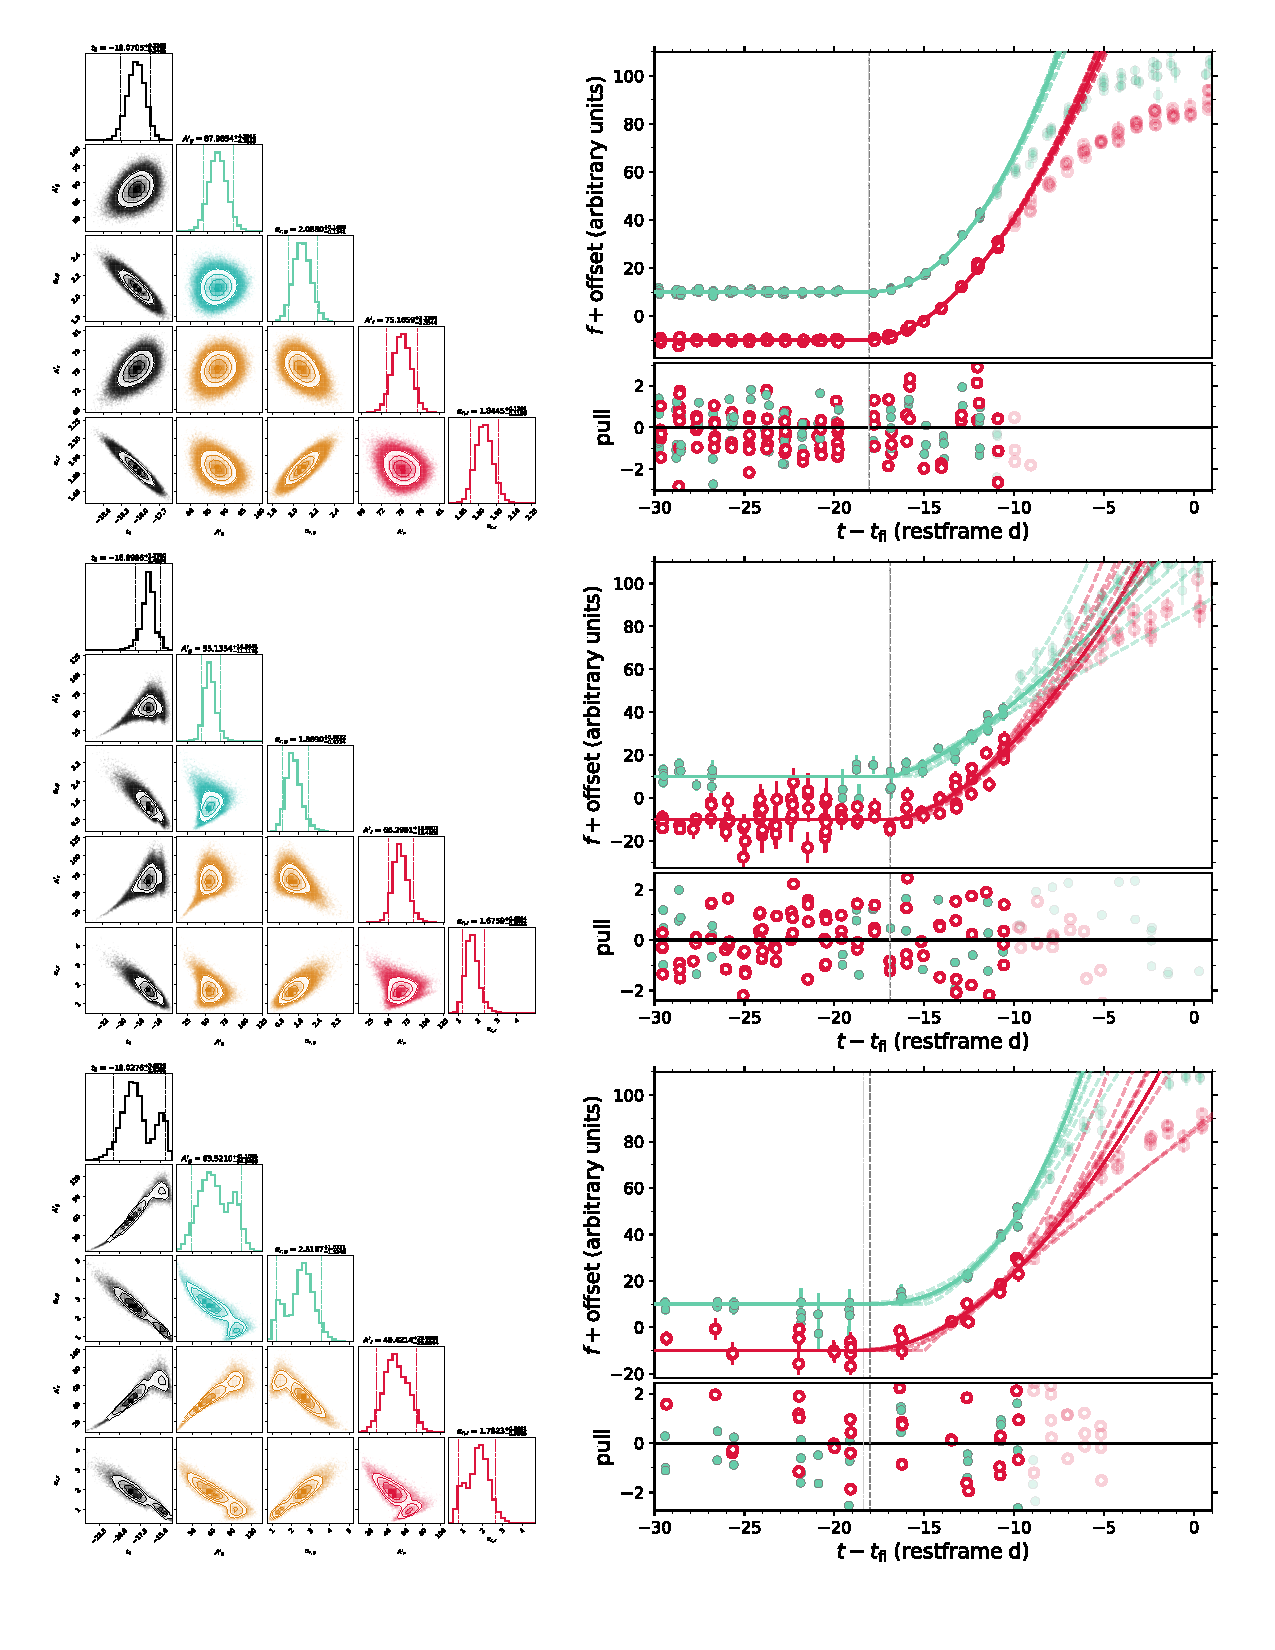
\includegraphics[width=5.75in]{./figures/corner_LC.pdf}
    %
    \caption{\textit{Left column}: Corner plots showing the posterior
    constraints on \tfl, $\alpha_g$, $\alpha_r$, and the respective constants
    of proportionality, $A_g$ and $A_r$ for ZTF18abgmcmv (top), a SN that is
    well fit by the model, ZTF18abukmty (middle), a typical SN in our sample,
    and ZTF18aazabmh (bottom), a SN that does not significantly constrain the
    model parameters. For clarity the $C_d$ and $\beta_d$ terms are excluded
    (in general they do not exhibit strong covariance with the parameters
    shown here as they are tightly constrained by the pre-SN observations).
    Marginalized one-dimentional distributions are shown along the diagonal,
    along with the median estimate and the 90\% credible region (shown with
    vertical dashed lines). \textit{Right column}: ZTF light curves of
    ZTF18abgmcmv (top), ZTF18abukmty (middle), and ZTF18aazabmh (bottom)
    showing the \gztf\ (filled, green circles) and \rztf\ (open, red circles)
    evolution of the SN in the month prior to the time of $B$-band maximum
    light (\tbmax). Observations included in the model fitting (i.e., those
    with $f \le 0.4 f_\mathrm{max}$) are dark and solid, while those that are
    not included are faint and semi-transparent. The maximum aposteriori
    model is shown via a thick solid line, while random draws from the
    posterior are shown with semi-transparent dashed lines. The vertical
    dashed line shows the median 1-D marginalized posterior value of \tfl,
    while the thin, light grey vertical line shows \tfl\ for the maximum
    aposteriori model. The bottom panel shows residuals relative to the
    maximum aposteriori model, where the factor $\beta_d$ has been included
    in the calculation of the residuals.}
    %
    \label{fig:corner_LC}
\end{figure*}

The light curves used to constrain the model parameters shown in the left
column of Figure~\ref{fig:corner_LC}, are shown in the right column of the
same figure. In addition to the data, we also multiple models based on random
draws from the posterior, and the residuals of the data relative to the
maximum aposteriori estimate from the MCMC sampling. From the top row of
Figure~\ref{fig:corner_LC}, it is clear that in the limit of high SNR, which
typically requires low redshift, and good sampling, it is possible to place
tight constraints on the model parameters. As expected, as the SNR decreases
(middle row) or the typical interval between observations increases (bottom
row), the data eventually reach the point where it is not possible to place
meaninful constraints on \tfl\ or $\alpha$. We visually examine posterior
models for each light curve and flag those that produce unreliable parameter
constraints. We use this subset of sources to identify SNe that should be
excluded from the full sample analysis described in \S\ref{sec:mean_parameters}
below (see Appendix~\ref{sec:qa}). These flagged sources are noted in
Table~\ref{tab:results}.

\section{The Mean Rise Time and Power-Law Index for SNe
Ia}\label{sec:mean_parameters}

Below we examine the results from our model fitting procedure to examine the
typical characteristics of \textit{normal} SNe Ia. We define normal as those
SNe that are suitable for cosmography, which can be
defined as $-2 \la X_1 \la 2$, where $X_1$ is the \texttt{SALT2} shape
parameter. Specifically within the context of our sample, this means we
exclude the SNe classified as SN\,1986G-like, SN\,2002cx-like, Ia-CSM, and
super Chandra explosions in \citet{Yao19} from the analysis below. These
events are specifically addressed in \S\ref{sec:rare}. Following the removal
of these events, 120 SNe remain in the sample.

\subsection{Mean Rise Time of SNe Ia}\label{sec:mean_rise}

From the marginalized 1D posteriors for \tfl, we can examine the typical rise
time for SNe Ia. The model given in Equation~\ref{eqn:flux_model} constrains
\tfl, yet we ultimately care about the rise time \trise. \tfl\ is measured
relative to \tbmax, the time of maximum light in the $B$-band, which itself
has some measurement uncertainty. An estimate of \trise\ must therefore
account for the uncertainties on both \tfl\ and \tbmax. To estimate \trise,
we use a Gaussian kernel density estimation (KDE) to approximate the 1-D
marginalized probability density function (PDF) for \tfl. The width of the
kernel is determined via cross validation and the KDE is implemented with
\texttt{scikit-learn} \citep{Pedregosa11}. The PDF is multiplied by $-1$ and
convolved with a Gaussian with the same variance as the uncertainties on
$t_\mathrm{B,max}$ to determine the final PDF for \trise. The cumulative
density function (CDF) of this PDF is used to determine the median and 90\%
credible region on \trise. There should be no covariance in the uncertainties
on \tfl\ and \tbmax, as these estimates are made using independent methods
and portions of the light curve, which is why we can convolve the
uncertainties in making the final estimation of \trise.

\begin{figure}
    \centering
    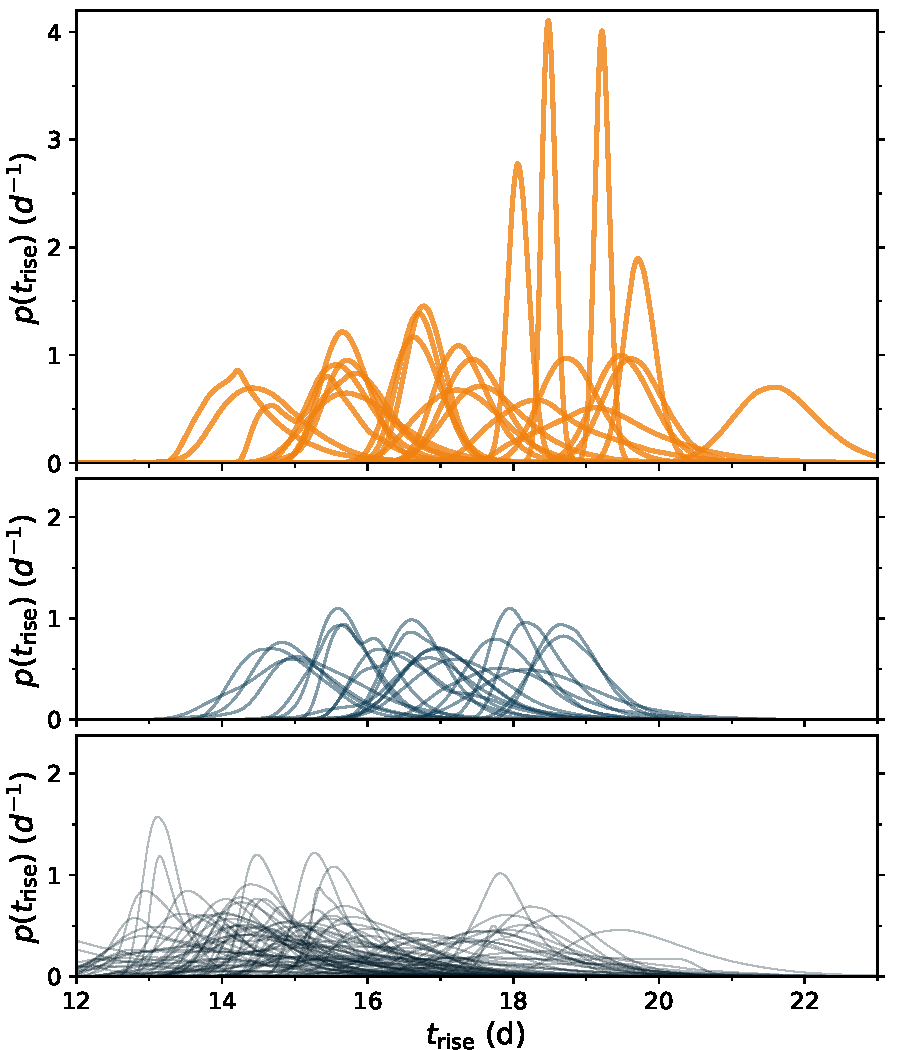
\includegraphics[width=1\linewidth]{./figures/rise_time.pdf}
    %
    \caption{Marginalized posterior distribution of the rise time
    $t_\mathrm{rise}$ for normal SNe Ia in our sample. The sample has been
    divded into three groups (as described in the text): thin grey lines show
    SNe from the unreliable group (see \ref{sec:qa}), dark blue lines show
    SNe from the reliable-$z_\mathrm{SN}$ group, and thick, orange lines show
    SNe reliable-$z_\mathrm{host}$ group. From the individual PDFs it is
    clear that there is no support for a single mean $t_\mathrm{rise}$ to
    describe every SN in the sample.}
    %
    \label{fig:rise_time}
\end{figure}

In Figure~\ref{fig:rise_time} we show the PDF for \trise\ for the 120 normal
SN in our sample. We highlight three subsets of the normal SNe in
Figure~\ref{fig:rise_time}, SNe with reliable model parameters (see~\ref{sec:qa}) and known host galaxy redshifts (hereafter the
reliable-$z_\mathrm{host}$ group), SNe with reliable model parameters and
unknown host galaxy redshifts (hereafter the reliable-$z_\mathrm{SN}$ group),
and SNe with unreliable model parameters (hereafter the unreliable group). 

Figure~\ref{fig:rise_time} shows that \trise\ for SNe in the unreliable group
are biased towards shorter rise times, which serves as additional
confirmation that data are insufficient for constraining the model parameters
for these sources. Figure~\ref{fig:rise_time} also shows that the individual
SNe do not tend towards a single mean value. If all SNe Ia could be described
with a single rise time, we could estimate that mean value by multiplying
together all of the PDFs shown in Figure~\ref{fig:rise_time}. The product of
the individual PDFs provides no support for a single rise time to describe
all SNe Ia (i.e., it is effectively equal to 0 everywhere). Thus, SNe Ia
follow a distribution of rise times, as has previously been reported (e.g.,
\citealt{Riess99a,Ganeshalingam11,Firth15,Zheng17a}).

As a population, SNe Ia have a mean \trise$ \approx 17.4$\,d, where we have
estimated this value by taking a weighted mean of the median value of the
\trise\ PDFs, with weights equal to the square of the inverse of the 68\%
credible region. The mean \trise\ increases to $\approx 18.0$\,d and
$18.3$\,d when considering only the reliable and reliable-$z_\mathrm{host}$
subsamples, respectively. The scatter, estimated via the sample standard
deviation, about these mean values is 1.8\,d, 1.6\,d, and 1.8\,d for the
full, reliable, and reliable-$z_\mathrm{host}$ subsamples, respectively.

\subsection{Mean Power-Law Index of the Early Rise}

We use a similar procedure to report the PDF of $\alpha_g$ and $\alpha_r$
under the assumption of a flat prior. The posterior samples shown in
Figure~\ref{fig:corner_LC} include a factor of $10^{-\alpha}$ following the
change of variables from $A$ to $A^\prime$. To remove this factor, we
estimate the 1-D marginalized PDF of $\alpha$ using a KDE as above. This PDF
is then divided by $10^{-\alpha}$, and then re-normalized to integrate to 1
on the interval from 0 to 10. This final normalized PDF provides an estimate
of $\alpha_g$ and $\alpha_r$ assuming a $\mathcal{U}(0,10)$ prior.

\begin{figure}
    \centering
    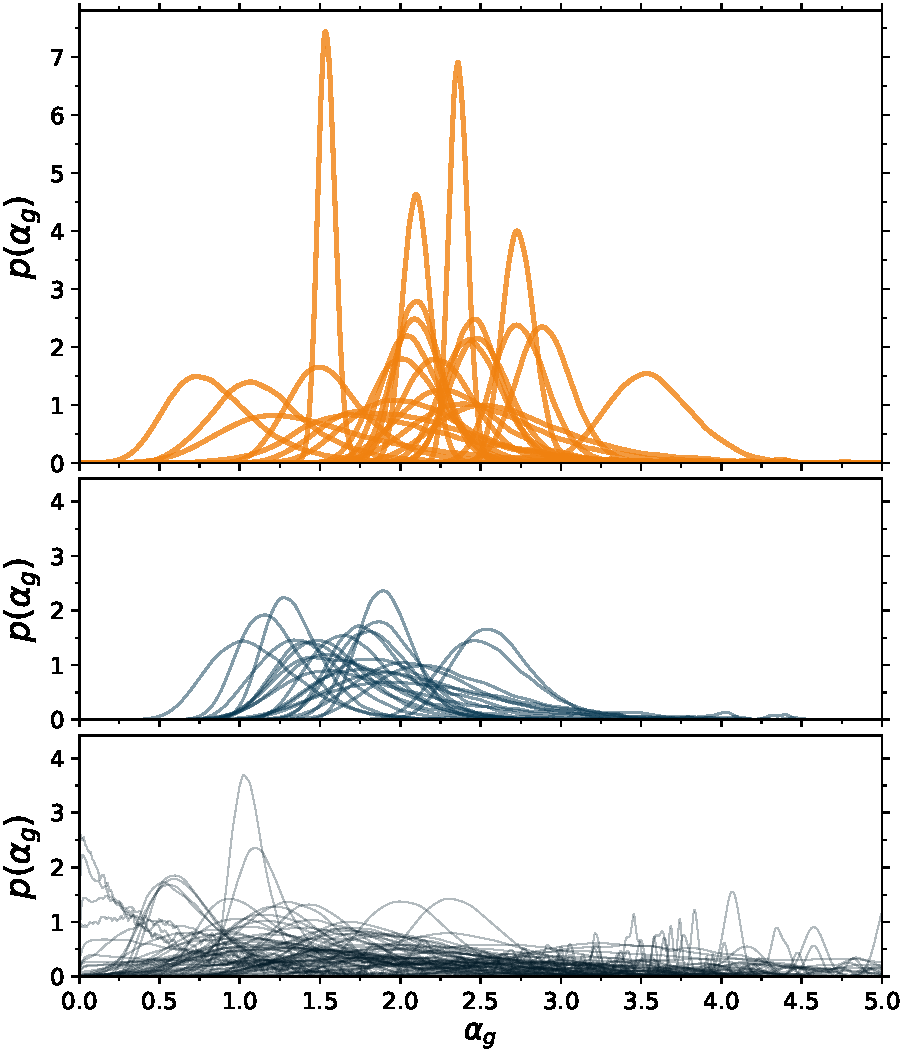
\includegraphics[width=1\linewidth]{./figures/alpha_g.pdf}
    %
    \caption{Marginalized posterior distribution of the rising power-law
    index in the \gztf-band $\alpha_g$ assuming a flat pqrior on $\alpha_g$
    for individual SNe in our sample. The color scheme is the same as in
    Figure~\ref{fig:rise_time}. While the
    density of the PDFs tends towards 2, as would be expected in the simple
    expanding fireball model, there is no support for a single mean power-law
    index to describe all SNe Ia.}
    %
    \label{fig:alpha_rise}
\end{figure}

The PDFs for $\alpha_g$ for normal SN Ia is shown in
Figure~\ref{fig:alpha_rise}. As in Figure~\ref{fig:rise_time}, we have
highlighted 3 subsamples of the data. The tightest constraints on $\alpha_g$
come from the reliable-$z_\mathrm{host}$ group, which are clustered around
$\alpha_g \approx 2$. There are, however, individual SNe within this subgroup
that provide support for $\alpha_g$ as low as $\sim$0.5 and as high as
$\sim$4. The data therefore suggest that $\alpha_g$ can take on a wide range
of values.

The weighted sample mean is $\alpha_g \approx 1.9$ for the normal SNe Ia in
the ZTF sample. This value increases to $\sim$2.1 when reducing the sample to
the reliable group or the reliable-$z_\mathrm{host}$ group. The scatter in the
population is 0.7, 0.5, and 0.6 for the full, reliable, and
reliable-$z_\mathrm{host}$ subsamples, respectively. For $\alpha_r$ the
weighted sample mean is $\sim$1.7 for the full sample of normal SNe Ia, which
increases to $\sim$1.9 and $\sim$2.0 for the reliable and
reliable-$z_\mathrm{host}$ subgroups, respectively. The scatter in $\alpha_r$
is 0.8, 0.5, and 0.5 for the full, reliable, and reliable-$z_\mathrm{host}$
subsamples, respectively. As noted below, there is an extremely tight
correlation between $\alpha_g$ and $\alpha_r$, and thus we do not show the
individual PDFs for $\alpha_r$.

In both the \gztf\ and \rztf\ filters the rising power-law index for the
initial evolution of the SN is remarkably close to 2, as would be expected in
the expanding fireball model. Similar results have been found in other studies
(e.g., \citealt{Conley06,Hayden10,Ganeshalingam11,Zheng17a}), though there are
some studies that have found that $\alpha$ is not consistent with 2
\citep{Firth15}. While the mean value of $\alpha$ is $\approx$2, it is
noteworthy that the PDF for several SNe in the reliable-$z_\mathrm{host}$
sample provide no support for $\alpha = 2$. As was the case for \trise, if we
multiply the individual PDFs of $\alpha_g$ or $\alpha_r$ together we find
there is no support for a single mean value of $\alpha$ capable of explaining
every SN in our sample. This suggests that models using a fixed value of
$\alpha$ are insufficient to explain the full population of normal SNe Ia.

\subsection{Mean Color Evolution}\label{sec:colors}

Here we examine the mean initial color evolution of SNe Ia, \textit{under the
assumption that the power-law model adopted in \S\ref{sec:model} is correct}.
This analysis does not address the initial colors of SNe Ia; for a more
detailed analysis of the early color and color evolution of SNe Ia see Paper
III in this series (Bulla et al.~2019, submitted).

Unlike \trise\ and $\alpha$, we do find evidence for a single mean value of
the early color evolution of SNe Ia, as traced by $\alpha_r - \alpha_g$. If
the early evolution in the \gztf\ and \rztf\ filters is a power-law in time,
then the \gztf\ $-$ \rztf\ colors will evolve $\propto (\alpha_r - \alpha_g)
\log_{10} (t - t_\mathrm{fl}$. Thus, negative values of $\alpha_r - \alpha_g$
result in a SN that gets bluer with time, positive values produce a SN that
gets redder, and $\alpha_r - \alpha_g = 0$ for a SN whose colors do not change.

\begin{figure}
    \centering
    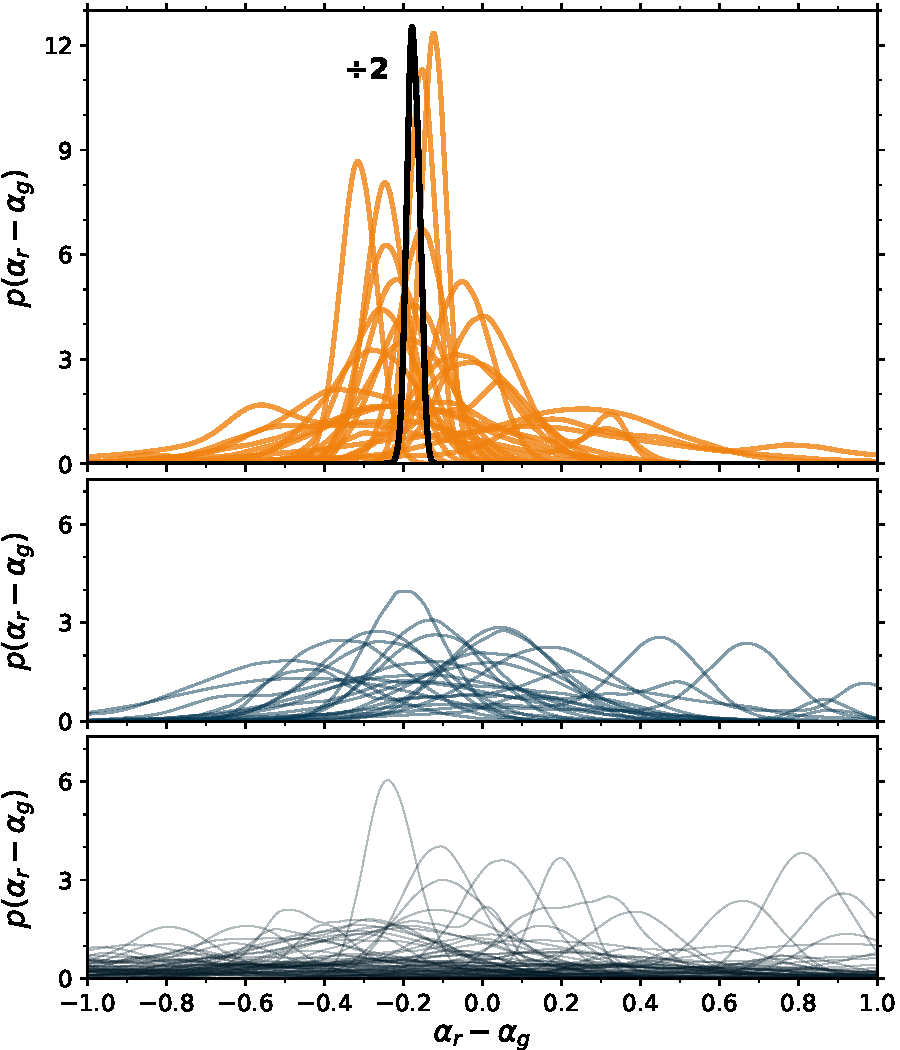
\includegraphics[width=1\linewidth]{./figures/delta.pdf}
    %
    \caption{Marginalized posterior distribution of the early color evolution of
    SNe Ia $\alpha_r - \alpha_g$ assuming flat priors on $\alpha_g$ and
    $\alpha_r$. The color scheme is the same as in Figure~\ref{fig:rise_time}.
    For SNe with reliable model parameters, there is support for a single mean
    value of $\alpha_r - \alpha_g \approx -0.17$, as shown by the thick, solid
    black line.}
    %
    \label{fig:delta}
\end{figure}

To estimate $\alpha_r - \alpha_g$ we use a similar procedure as above,
however, we need to estimate the marginalized joint posterior on $\alpha_g$
and $\alpha_r$, $\pi(\alpha_g,\alpha_r \mid t_\mathrm{fl}, A^\prime_b,
\beta_d)$, in order to correct the posterior estimates for the priors on
$\alpha$. To do so we estimate the 2D joint posterior via a Gaussian KDE,
correct this distribution for the priors on $\alpha_g$ and $\alpha_r$, and
then obtain random draws from this distribution to estimate the 1D
marginalized likelihood estimates on $\alpha_r - \alpha_g$. The distribution
of this parameter for individual SNe is shown in Figure~\ref{fig:delta}.

Unlike the estimates for \trise\ and $\alpha$ alone, $\alpha_r - \alpha_g$ is
clearly clustered around a value of $\sim{-0.2}$ for the reliable subset of
model parameters. Multiplying these likelihoods together produces support for a
single mean value of $\alpha_r - \alpha_g = -0.169 \pm 0.015$, where the
uncertainties on that estimate represent the 90\% credible region. The
distribution on this mean is shown as the thick, solid black line in
Figure~\ref{fig:delta}. A mean value of $\alpha_r - \alpha_g$ means that the
typical normal SN Ia becomes bluer in the days after explosion. Such an
evolution makes sense for an optically thick, radioactively heated, expanding
ejecta. There are, however, clear examples of individual SNe that do not exhibit
this behavior (e.g., SN\,2017cbv and iPTF\,16abc;
\citealt{Hosseinzadeh17,Miller18}), meaning this mean behavior is not
perscriptive for every SN Ia. Finally, we note that the above results exclude
SNe from the unreliable group, and their inclusion would remove any support for
a single mean value of $\alpha_r - \alpha_g$. This is largely due to a small
handful of events that feature extreme values of $\alpha_r - \alpha_g$ because
there are gaps in the observational coverage of one of the two filters (see the
upper right panel of Figure~\ref{fig:model_parameters}).

\section{Population correlations}

In addition to looking at the typical values of \trise\ and $\alpha$ for SNe
Ia, we also examine the correlations between these parameters, as well as how
they change with redshift $z$. These correlations may reveal details about the
explosion physics of SNe Ia (for example, if strong mixing in the SN ejecta
leads to low values of $\alpha$, as found in \citealt{Piro16}, then any
correlations with $\alpha$ may be related to ejecta mixing). Alternatively,
these correlations may reveal inadequacies in the model. If the model
parameters are correlated with redshift, that could be evidence for the cosmic
evolution of SNe Ia progenitors.

The correlation between $t_\mathrm{rise}$, $\alpha_g$, $\alpha_r$, and $z$ is
shown in Figure~\ref{fig:model_parameters}. We do not show the correlation
between $\alpha_r$ and $z$ or between $\alpha_g$ and \trise, as this
information is effectively redundant given the tight correlation between
$\alpha_g$ and $\alpha_r$ (top right panel of
Figure~\ref{fig:model_parameters}).

\begin{figure*}
    \centering
    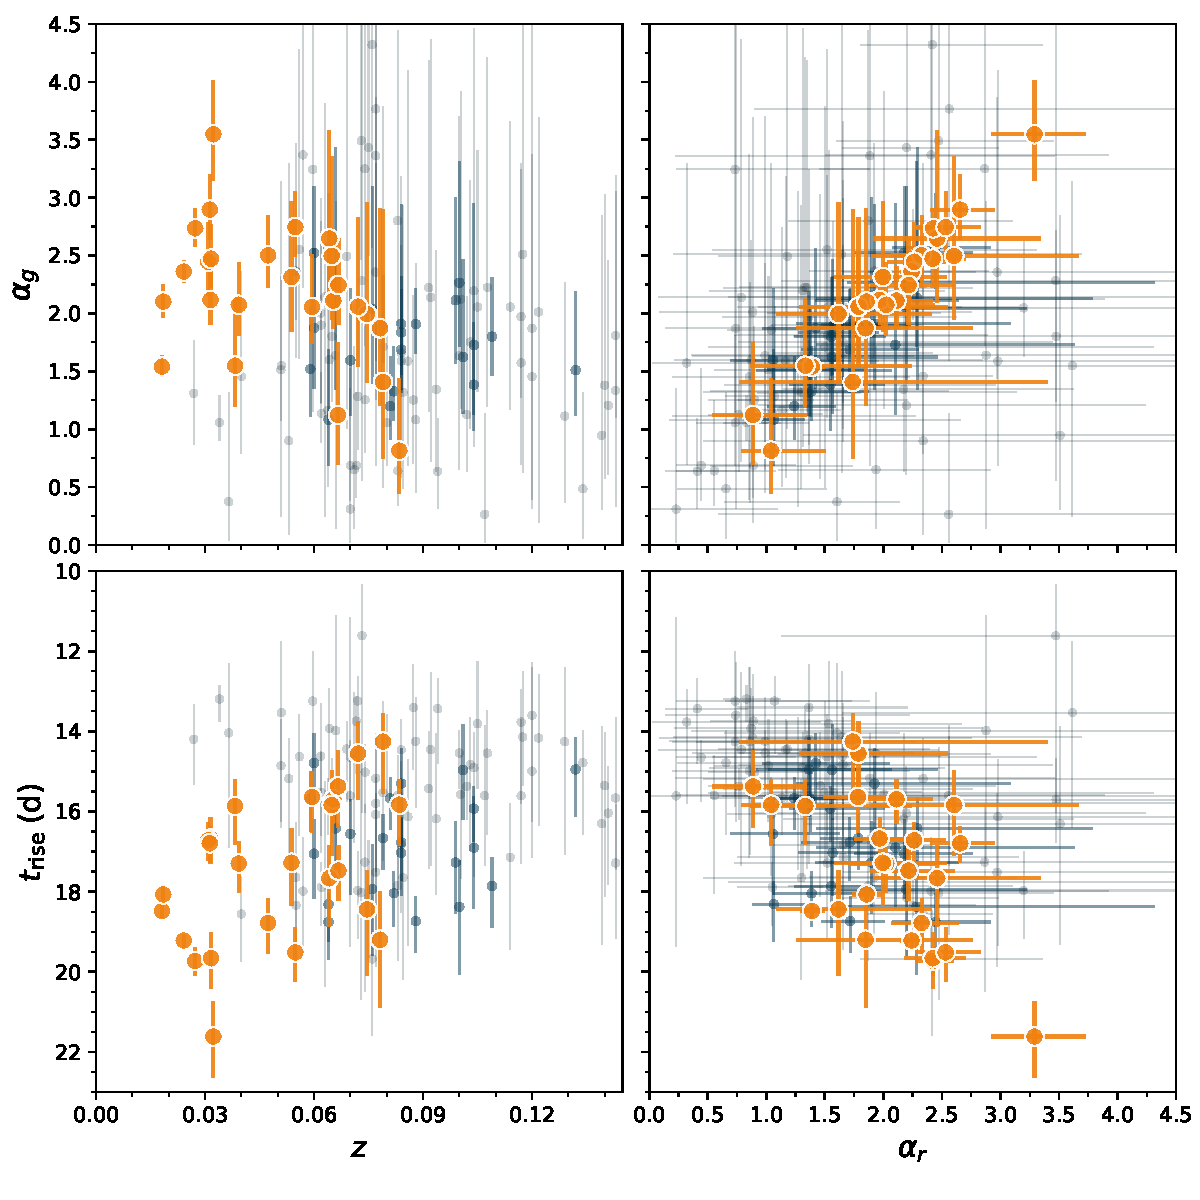
\includegraphics[width=6in]{./figures/param_correlations.pdf}
    %
    \caption{Correlation between redshift $z$, SN rise time
    $t_\mathrm{rise}$, and the power-law index in the \gztf\ and \rztf\
    filters, $\alpha_g$ and $\alpha_r$, respectively. We do not show
    $\alpha_r$ vs.~$z$ or $t_\mathrm{rise}$ vs.~$\alpha_g$, as these would
    largely be redundant given the very strong correlation between $\alpha_g$
    and $\alpha_r$ (upper right panel). The sample has been divded into three
    groups: small, light grey circles show SNe with unreliable fits (see
    \ref{sec:qa}), dark blue circles show reliable fits where the host
    galaxy redshift is not known, and large orange circles show SNe with
    reliable fits with known host galaxy redshifts. The plots show that
    redshift is correlated with both $t_\mathrm{rise}$ and $\alpha_g$, which
    would only be expected is SNe Ia undergo significant evolution from $z
    \approx 0.1$ to $0$. We later show this to be the result of a systematic
    selection effect (see text for further details). }
    %
    \label{fig:model_parameters}
\end{figure*}

\subsection{Correlation Between $\alpha_g$ and $\alpha_r$}

The most striking, and also least surprising, feature in
Figure~\ref{fig:model_parameters} is the tight correlation observed between
$\alpha_g$ and $\alpha_r$. This result is unsurprising because the \gztf\
and \rztf\ filters sample adjacent portions of the SN spectral energy
distribution (SED), and thus the evolution should be nearly identical in the
two filters. SNe with reliable model parameters follow a tight locus around
$\alpha_g - \alpha_r \approx 0.1$, with the only major outliers from this
relation being SNe in the unreliable group (for further discussion of the
early \gztf\ $-$ \rztf\ color evolution of this sample see M.~Bulla et al.
2019).

The Spearman rank-ordered correlation coefficient for $\alpha_g$
and $\alpha_r$ is highly significant for the entire population ($\rho >
0.5$), confirming what can clearly be seen by eye. Restricting the sample to
SNe with reliable model parameters increases the significance of the
correlation dramatically ($\rho > 0.9$). Thus, knowledge of the power-lax
index in either filter provides a strong predictor for the power-law index
in the other filter, which, again is not a surprising result.

\subsection{Correlations with Redshift -- Systematics, Not Cosmic Evolution}\label{sec:redshift_correlations}

While less prominent, Figure~\ref{fig:model_parameters} additionally shows
that both \trise\ and $\alpha$ are correlated with redshift. This result is
somewhat surprising: naively, it suggests some form of cosmic evolution in SNe
Ia, with SNe at $z \approx 0.08$ having rise times that are several days
shorter than SNe at $z \approx 0.02$. The small range of redshifts in our
sample, and several previous studies (e.g., \citealt{Conley06} \todo{add Riess ref?}),
render this naive explanation in doubt. Instead, this correlation can be
understood as the result of building a sample from a flux-limited survey.

Given the fixed depth of ZTF observations ($g_\mathrm{lim} \la 21.5$\,mag;
\citealt{Masci19,Bellm19}), SNe at progressively higher redshifts will be
discovered later and later in their evolution. The large degeneracies in the
model presented in Equation~\ref{eqn:flux_model}, namely between \tfl, $A$,
and $\alpha$, allow for a great deal of flexibility when fitting the data. In
particular, to match the first detection ($\mathrm{SNR} \ga 3$) in the light
curve, it is possible to adjust \tfl\ to successively larger values (i.e.,
shorter rise times), while decreasing $A$ and $\alpha$, such that \tfl\ occurs
around the epoch of first detection. 

We illustrate this behavior in Figure~\ref{fig:high_z_systematic}, which shows
the inferred rise time for four low-$z$ SNe had they been observed at
successively higher redshifts. To simulate these SNe at higher redshift we
make the (over-simplified) assumption that all detections are in the
sky-background dominated regime, and therefore in any given epoch the
$\mathrm{SNR} \propto d_L^{-2}$, where $d_L$ is the luminosity distance to the
SN. Under this assumption, multiplying the uncertainties by the ratio of the
square of the simulated distance to the square of the actual distance provides
the SNR for the SN at the simulated redshift.\footnote{Following
\citet{Yao19}, we adopt a flat $\Lambda$CDM cosmology with $H_0 =
73.24$\,km\,s$^{-1}$\,Mpc$^{-1}$ \citep{Riess16} and $\Omega_m = 0.275$
\citep{Amanullah10} to calculate $d_L$ for the SNe.} Using these increased
uncertainties, we randomly resample the observed flux values from a normal
distribution with mean equal to the original flux and variance equal to the
scaled uncertainty squared. This resampling is necessary, as the $\beta_d$
term in Equation~\ref{eqn:flux_model} would otherwise reverse the increase in
the uncertainties when maximizing the posterior. We then fit the noisier
simulated data with the same procedure described in Section~\ref{sec:model}.
This procedure is repeated at redshifts of $z = 0.05$, 0.075, 0.1, and 0.015.
Only the models that converge are shown in Figure~\ref{fig:high_z_systematic}.

\begin{figure}
    \centering
    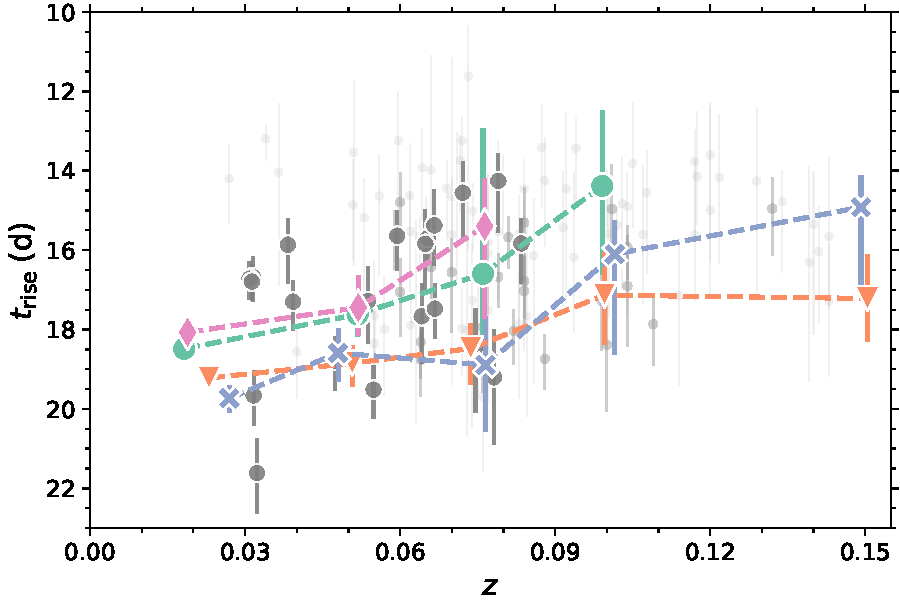
\includegraphics[width=1\linewidth]{./figures/high_z_systematic.pdf}
    %
    \caption{Same as the bottom left panel of
    Figure~\ref{fig:model_parameters}, though all SNe are shown in grey. The
    large green circle, magenta diamond, orange triangle, and purple $X$ show
    how marginalized posterior estimates of \trise\ change as the four lowest
    redshift SNe are observed at $z = 0.05$, 0.075, 0.1, and 0.015 (see text
    for further details). \trise\ clearly decreases with increasing redshift,
    showing that the observed correlation between these parameters is due to
    the flux-limited ZTF search for SNe, and not cosmic evolution.}
    %
    \label{fig:high_z_systematic}
\end{figure}

The results of this simulation are clear: as the SN redshift increases, the
rise time correspondingly decreases. This result is simple to understand as
higher redshift SNe will not be detected until later in their evolution. A
stronger prior on any of the model parameters would help to combat this
effect, though as previously discussed we avoid strong priors due to the wide
range of $\alpha$ and \tfl\ that has been reported in the literature. This
effect also explains the correlation seen in the bottom right panel of
Figure~\ref{fig:model_parameters}. SNe detected later in their evolution will
be evolving less rapidly as the rate of change in brightness continually
decreases until the time of maximum light. Hence, a later detection provides a
lower value of $\alpha$. Indeed, a re-creation of
Figure~\ref{fig:high_z_systematic} showing $\alpha_g$ instead of \trise\ shows
$\alpha_g$ decreasing with increasing redshift. Thus, the observed
correlations with redshift seen in Figure~\ref{fig:model_parameters} can be
entirely understood as the result of ZTF being a flux-limited survey.

The implications of this result have consequences well beyond the ZTF sample
discussed here. Essentially all SN surveys are flux-limited, meaning the
systematics associated with redshift will affect any efforts to determine
\trise\ or $\alpha$ in those data as well. The inclusion of higher-redshift
SNe in the sample will, on average, bias estimates of \trise\ and $\alpha$ to
lower values. Even more concerning is the possibility that this trend may
continue to very low redshifts ($z \ll 0.01$). The paucity of SNe in this
redshift range, due to the relatively small volume probed, make it difficult
to test for such an effect. Due to the systematic identified here, it may be
the case that the rise time, and by extension also $\alpha$, are
underestimated for every SN in the literature. Detailed simulations with
realistic SN light curves are needed to test this posibility.

\subsection{Correlations with Light Curve Shape}

A defining characteristic of SNe Ia is that they can be described by a
relatively simple luminosity-shape relation \citep{Phillips93}, which enables
them to be used as standardizable candles. We examine the correlation between
light curve shape, in this case the \texttt{SALT2} $X_1$ parameter, and the SN
rise time and $\alpha$ in Figure~\ref{fig:shape_correlations}. There is a
clear correlation between shape and \trise, a result that has been reported
previously (e.g., \citealt{Riess99a,Firth15,Zheng17a}). This result is also
completely unsurprising as the $X_1$ shape parameter accounts for the width of
both the SN rise and decline, and therefore, by definition should be
correlated with the rise time. The middle and right panels of
Figure~\ref{fig:shape_correlations} divide the reliable-$z_\mathrm{host}$
group into low ($z < 0.06$) and high ($z \ge 0.06$) redshift bins. From these
panels it is clear that some of the scatter in the $X_1$-\trise\ plane is the
result of the redshift bias discussed in \S\ref{sec:redshift_correlations}, as
higher redshift SNe have shorter rise times at fixed $X_1$. A correction for
this redshift effect would reduce the overall scatter seen in the lower panels
of Figure~\ref{fig:shape_correlations}.

\begin{figure*}
    \centering
    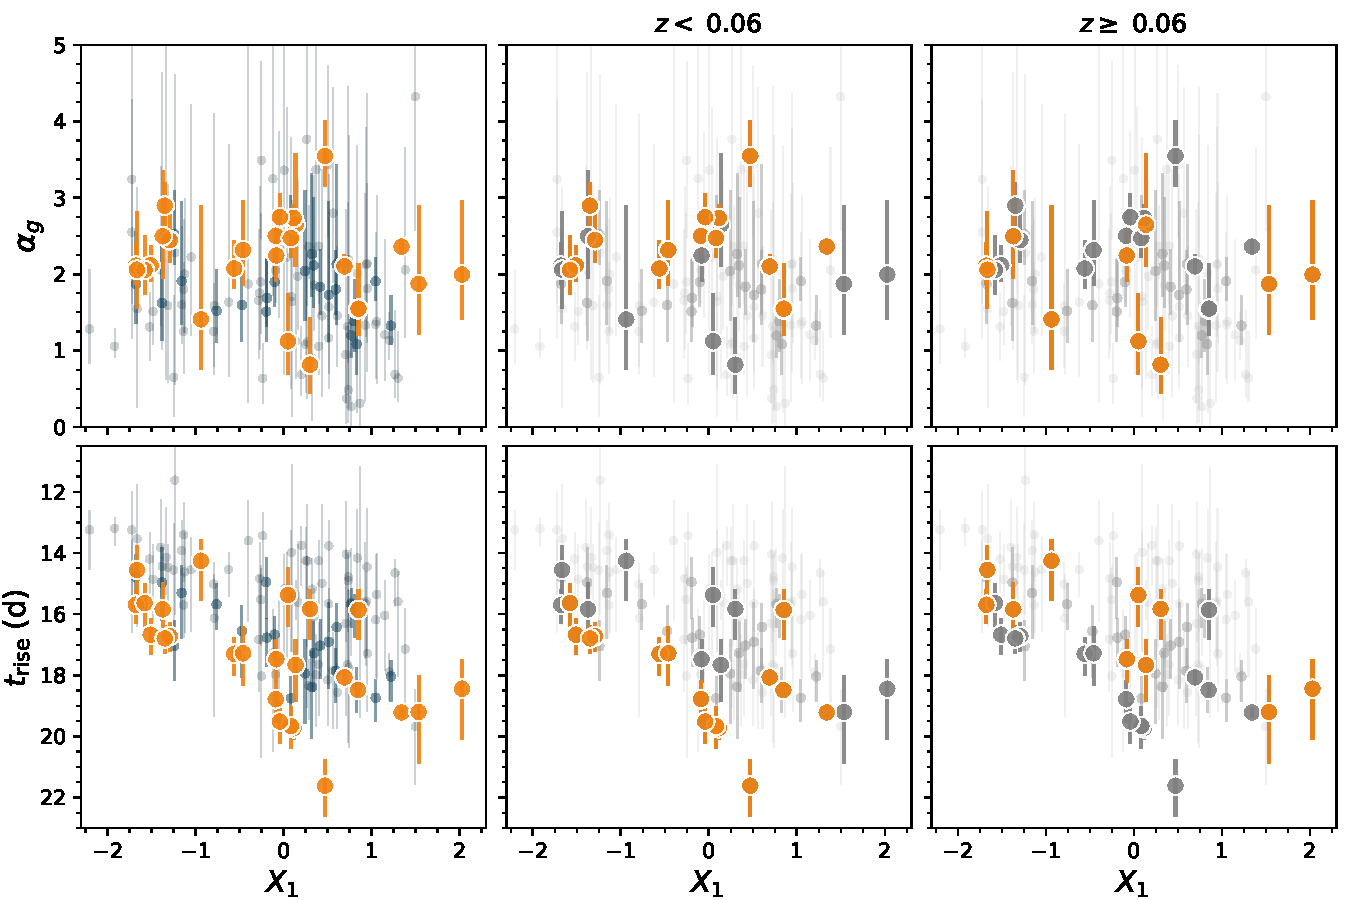
\includegraphics[width=6in]{./figures/shape_correlations.pdf}
    %
    \caption{Correlation between the \texttt{SALT2} $X_1$ shape parameter and
    $\alpha_g$ (top row) and \trise\ (bottom row). Symbols are the same as
    Figure~\ref{fig:model_parameters}. For clarity, the uncertainties on $X_1$
    are not shown. \trise\ shows a strong correlation with $X_1$, while there
    is no correlation between $\alpha_g$ and $X_1$. The middle and right
    panels highlight reliable-$z_\mathrm{host}$ SNe at low, $z < 0.06$, and
    high, $z \ge 0.06$, redshift, respectively. Dividing the sample into
    different redshift bins shows that most of the observed scatter between
    $X_1$ and the model parameters is due to redshift and not intrinsic
    scatter. }
    %
    \label{fig:shape_correlations}
\end{figure*}

\begin{figure*}
    \centering
    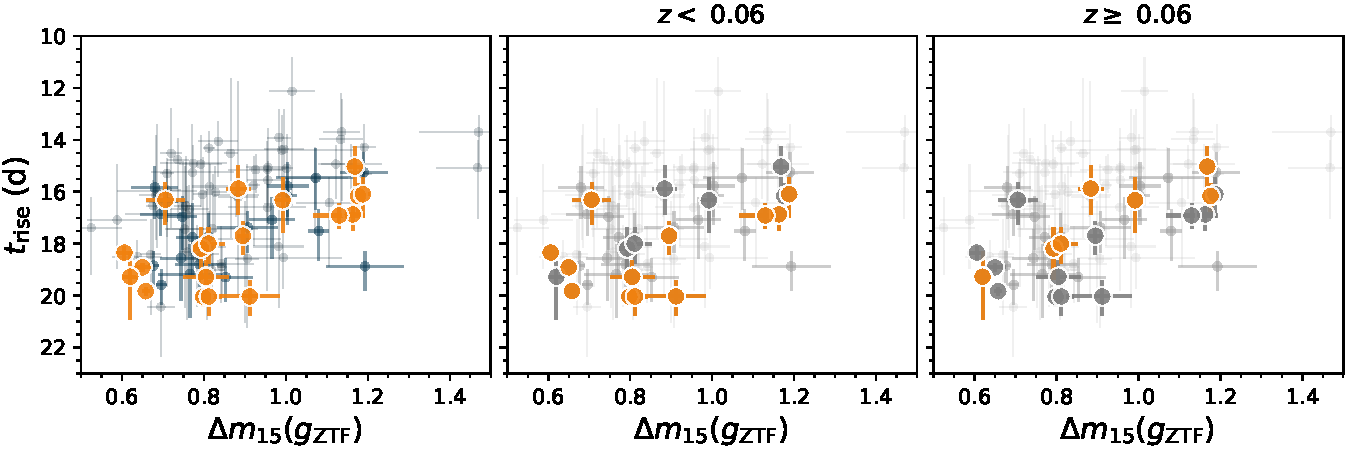
\includegraphics[width=6in]{./figures/dm15_rise.pdf}
    %
    \caption{Correlation between $\Delta m_{15}(g_\mathrm{ZTF})$ and \trise.
    Symbols are the same as Figure~\ref{fig:model_parameters}. There is a clear
    correlation between the rise and decline times of SNe Ia. Some of the
    scatter in the relationship between these parameters can be explained as a
    result of the redshift effect discussed in
    \S\ref{sec:redshift_correlations}. \todo{remake figure with less white
    space}}
    %
    \label{fig:dm15}
\end{figure*}

We compare independent measurements of the rise time and decline of SNe Ia in
Figure~\ref{fig:dm15}, which shows the correlation between \trise\ and $\Delta
m_{15}(g_\mathrm{ZTF})$, the observed decline in magnitudes of the \gztf\
light curve between the time of maximum light and 15\,d later. $\Delta
m_{15}(g_\mathrm{ZTF})$ is measured via low-order polynomial fits to the
\gztf\ photometry from phase $= -5$ to $+20$\,d. Thus, unlike our measurements
of $X_1$, the $\Delta m_{15}(g_\mathrm{ZTF})$ values that we infer utilize
entirely different observations than those used to estimate \trise. For 15 of
the 127 SNe in our sample this measurement is not possible due to an
insufficient number of observations in the defined window. We additionally
exclude 6 SNe from Figure~\ref{fig:dm15} where the relative uncertainty on
$\Delta m_{15}(g_\mathrm{ZTF})$ is greater than 25\%. Figure~\ref{fig:dm15}
shows that, on average, slowly declining SNe (i.e., smaller values of $\Delta
m_{15}(g_\mathrm{ZTF})$) have longer rise times, confirming the trend shown in
Figure~\ref{fig:shape_correlations}. Furthermore, Figure~\ref{fig:dm15}, like
Figure~\ref{fig:shape_correlations}, shows that at least some of the scatter
in this relation can be explained as a redshift effect because SNe at higher
redshift have shorter rise times, on average, for a fixed value of $\Delta
m_{15}(g_\mathrm{ZTF})$.

The observed correlation between the rise time and the SN decline stands in
contrast to what was found in \citet{Hayden10}, where the slowest declining
SNe are among the fastest risers, and a few fast-declining SNe have long rise
times. This particular result may be understood in the context described in
\S\ref{sec:redshift_correlations}. Slowly declining SNe are more luminous, and
therefore will, on average, be found at higher redshifts than rapidly
declining events in a flux limited survey. As
Figure~\ref{fig:high_z_systematic} shows, for SNe all discovered by the same
survey, the rise times are underestimated for higher redshift events. Indeed,
such an effect is seen in the ZTF sample, as illustrated in the 3 right
columns of Figure~\ref{fig:shape_correlations}. If the
reliable-$z_\mathrm{host}$ subsample is divided in redshift bins, it is clear
that, at fixed values of $X_1$, the corresponding value of \trise\ decreases
as the redshift increases. This bolsters the arguments in
\S\ref{sec:redshift_correlations} that there is a systematic error in the
estimate of \trise\ due to redshift, and means that the intrinsic scatter in
the relation between $X_1$ and \trise\ is much smaller than the observed
scatter seen in Figure~\ref{fig:shape_correlations}.

There is no strong correlation between $\alpha$ and $X_1$
(Figure~\ref{fig:shape_correlations}). The Spearman rank-ordered correlation
for these two parameters is $\rho \approx -0.2$ whether looking at $\alpha_g$
or $\alpha_r$, or whether considering the full sample, the reliable group, or
the reliable-$z_\mathrm{host}$ group. Subdividing the
reliable-$z_\mathrm{host}$ group by redshift shows the same trend that was
identified in Figure~\ref{fig:model_parameters}: higher redshift SNe have
smaller values of $\alpha$ on average for the reliable-$z_\mathrm{host}$ group.

\section{Strong Priors}\label{sec:strong_priors}

\subsection{Fixing $\alpha = 2$}

In our previous effort to model the early evolution of SNe Ia we adopted a
flexible model (hereafter the ``uninformative prior'') allowing $\alpha$ and
\tfl\ to simultaneously vary despite theoretical \citep{Arnett82,Riess99a} and
observational \citep{Conley06,Hayden10,Ganeshalingam11} evidence that $\alpha$
is consistent with $2$. Here we alter the model by fixing $\alpha_g = \alpha_r
= 2$ (hereafter the ``$\alpha = 2$ prior''), and explore how this decision
changes the results described in the previous sections. This decision is
equivalent to placing an infinitely strong prior on the value of
$\alpha$.\footnote{Strictly enforcing $\alpha_g = \alpha_r$ imposes
non-physical structure on the models, as this condition effectively implies
that there is no change in the $g - r$ colors during the initial rise of the
SN. This is clearly observed not to be the case in many SNe
(\S\ref{sec:colors}; see also Paper III in this series, Bulla et al.\ 2019,
submitted).}

The distribution of rise time PDFs using the $\alpha = 2$ prior is shown in
Figure~\ref{fig:tsquared_rise}. Adopting this strict prior significantly
reduces the flexibility of the model. One consequence of this choice is that
visual inspection of the posterior predictive flux values reveals that there
are far fewer SNe with unreliable model parameters. When using the $\alpha =
2$ prior, we only flag SNe with an extrapolated flux using the maximum
aposteriori model parameters $< 0.9 f_\mathrm{max}$ at \tbmax\ as having
unreliable model parameters. From this criterion only 5 SNe are flagged as
having unreliable model parameters.

\begin{figure}
    \centering
    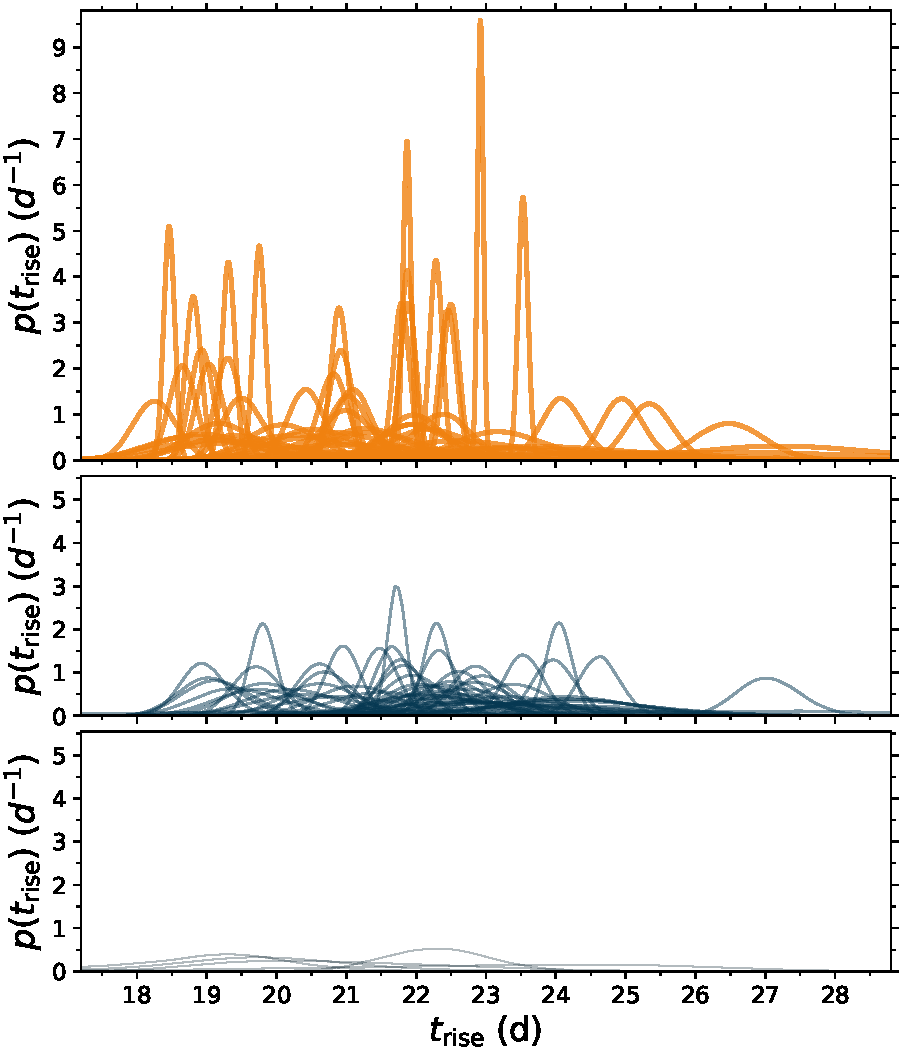
\includegraphics[width=1\linewidth]{./figures/tsquared_rise_time.pdf}
    %
    \caption{Same as Figure~\ref{fig:rise_time}, showing the resulting PDFs for
    the $\alpha = 2$ prior. Note that the definition for reliable model
    parameters with the $\alpha = 2$ prior is different from that described in
    \ref{sec:qa}, as described in the text. As was the case when $\alpha$ is
    allowed to vary, there is no support for a single mean $t_\mathrm{rise}$ to
    describe every SN in the sample. The $\alpha = 2$ prior results in rise
    times that are $\sim$3\,d longer on average.}
    %
    \label{fig:tsquared_rise}
\end{figure}

Figure~\ref{fig:tsquared_rise} shows distinct differences in the distribution
of rise times relative to Figure~\ref{fig:rise_time}. There are far more SNe
with narrow PDFs for \trise\ when adopting the $\alpha = 2$ prior.
Furthermore, the typical rise time is $\sim$3\,d longer than what is inferred
from the uninformative priors. Nevertheless, as is the case when adopting
uninformative priors, there is no support for a single mean rise time to
describe all SNe Ia. We find a population mean \trise\;$\approx 21.0$\,d,
using the same method described in \S\ref{sec:mean_rise}. This mean value does
not significantly change when considering the full, reliable, or
reliable-$z_\mathrm{host}$ samples. The population scatter about this mean
value is 1.7\,d, 1.8\,d, and 2.0\,d for the full, reliable, and
reliable-$z_\mathrm{host}$ subsamples, respectively. Another consequence of
adopting the $\alpha = 2$ prior is that 3 SNe in the sample have rise times
that are consistent with 28\,d, which is considerably longer than the rise
times inferred in any previous study of normal SNe Ia.

In Figure~\ref{fig:tsquared_z_evolution} scatter plots of the inferred value
of \trise\ when adopting the $\alpha = 2$ prior are shown against both
redshift and $X_1$. The previously observed correlation between \trise\ and
redshift disappears when adopting $\alpha = 2$. The Spearman rank-order
correlation coefficient for these two parameters is $\rho \la 0.2$ when
considering any of the full, reliable, or reliable-$z_\mathrm{host}$
subsamples. The model is, in effect, no longer flexible enough to
systematically adjust \tfl\ to be approximately equal to the epoch of first
detection. The removal of this particular bias provides a benefit for fixing
$\alpha = 2$.

\begin{figure*}
    \centering
    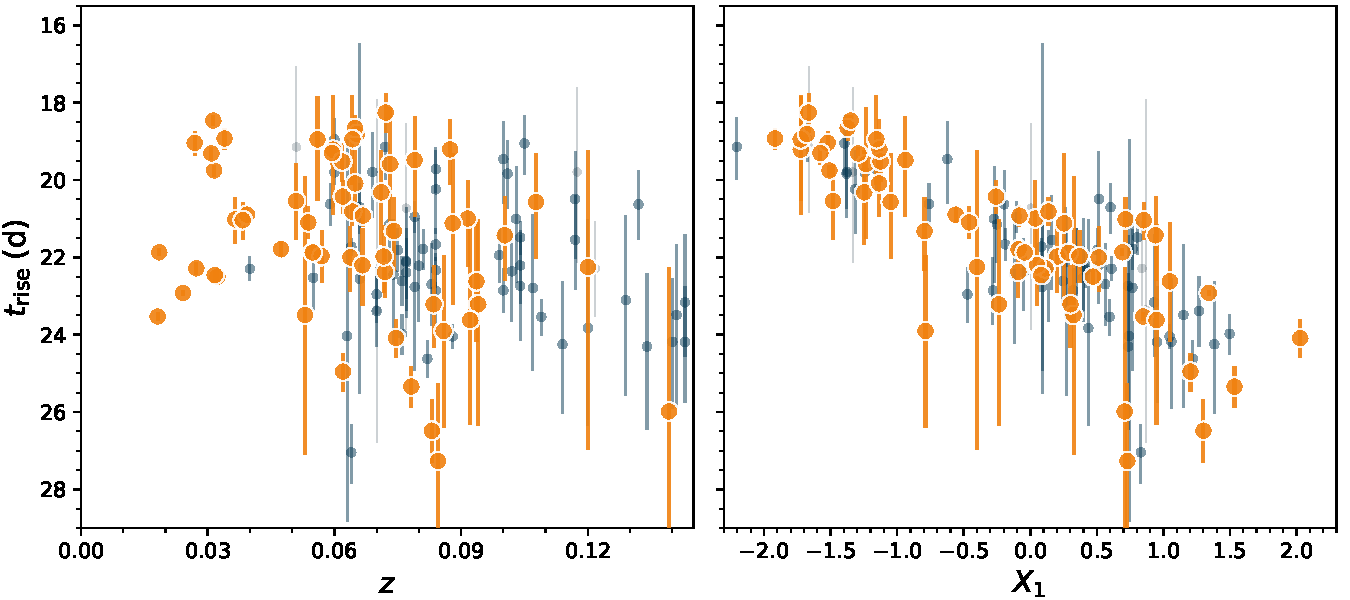
\includegraphics[width=6in]{./figures/trise_z_tsquared.pdf}
    %
    \caption{Correlation between \trise\ and redshift (left) and $X_1$ (right)
    when adopting the $\alpha = 2$ prior on the model for early emission from
    SNe Ia. The use of this strict prior removes the previously observed bias
    that resulted in shorter rise times being inferred at higher redshifts. A
    consequence of the removal of this bias is a reduction in the obsered
    scatter between \trise\ and $X_1$.}
    %
    \label{fig:tsquared_z_evolution}
\end{figure*}

There is far less scatter in the correlation between $X_1$ and \trise\ when
adopting the $\alpha = 2$ prior. The reduction in this scatter intuitively
makes sense, given that it was due, at least in part, to the redshift bias in
measuring \trise\ (\S\ref{sec:redshift_correlations}). Reducing, or possibly
fully removing, that bias by adopting the $\alpha = 2$ prior allows a directly
estimate the rise time from $X_1$ with a typical scatter $< 1$\,d. If
relatively high precision measurements of \trise\ can be directly inferred
from $X_1$, it would dramatically increase the sample of SNe Ia with measured
rise times, as extremely early observations ($t < -10$\,d) would no longer be
required given that $X_1$ can be inferred solely from observations around and
post-peak maximum light.

\subsection{Model Selection}\label{sec:dic}

In adopting two very different priors that, in turn, produce significantly
different posteriors, we are naturally left with the question: which model is
better? To some extent, the answer to this question rests with every individual
as the prior quantifies one's a priori belief about the model parameters. We
posit that it is extremely unlikely that thermonuclear explosions all
identically produce $\alpha = 2$ across a multitude of filters. Thus, adopting
$\alpha = 2$ is very likely an overconfident position that produces slightly
biased inference as a result.

Alternatively, we can address the question of which model is best via the use
of model selection techniques based on information criteria. In our initial
fit of the SN light curves we effectively included additional parameters in
the model by allowing $\alpha$ to vary. Thus, for individual SNe, we can
compare the trade off between increasing the model complexity relative to the
overall improvement in the model fit to the data, in order to determine which
model is superior. Following \citet{Spiegelhalter02}, we define the deviance
$D$ as
%
$$D(\theta) = -2 \ln (p(x\mid \theta)) + C,$$
%
where $\theta$ are the model parameters, $x$ are the observations, $p(x\mid
\theta)$ is the likelihood, and $C$ is a constant that will drop out following
model comparison. From here, the effective number\footnote{We adopt the
Deviance Information Criterion, as opposed to the Akaike or Bayesian
Information Criteria because our model includes many nuissance parameters that
we ultimately marginalize out of our final inference. The DIC more natually
accounts for these marginalized parameters.} of model parameters $p_D$ can be
calculated as:
%
$$p_D = \langle D(\theta) \rangle - D(\langle \theta \rangle),$$
%
where $\langle D(\theta) \rangle$ is the mean posterior value of the deviance,
and $D(\langle \theta \rangle)$ is the deviance of the mean posterior model
parameters. We then define the deviation information criterion (DIC) as:
%
$$\mathrm{DIC} = p_D + \langle D(\theta) \rangle.$$
Smaller values of  the DIC are  preferred to larger values.

Following \citet{Jeffreys61} we consider SNe with
%
$$\exp(\mathrm{DIC}_{\alpha2} - \mathrm{DIC}_\mathrm{flat})/2) \ge 30,$$
%
where $\mathrm{DIC}_{\alpha2}$ is the DIC for the $\alpha = 2$ prior and
$\mathrm{DIC}_\mathrm{flat}$ is the DIC for the uninformative prior, to
exhibit a very strong preference for the uniformative prior. Of the 127 SNe in
our sample, including the 7 SNe that are not considered normal SNe Ia, only 29
show a strong preference for the uniformative prior. Of these 29, however, 16
are part of the unreliable group, and indeed, visual inspection shows that
these SNe have very few detections after \tfl. In these cases the uniformative
prior leads to small values of $\alpha$ that effectively perfectly match the
few detections of the SN (see e.g., Figure~\ref{fig:biggap_lc}). The other 13
SNe constitute the lowest redshift SNe in our sample with small, if any, gaps
in the observational coverage.

These results suggest that the preferred value of \tfl\ should come from the
$\alpha = 2$ prior for the majority of the SNe in our sample, with the
exception of the 13 SNe where the uniformative prior is preferred according to
the DIC and the model parameters associated with that prior are considered
reliable. This approach is how we define the distribution of \tfl\ in Paper
III of this series (M.~Bulla et al.~2019, submitted).

\section{A Volume Limited Sample of Normal SNe Ia}\label{sec:volume_limited}

The ZTF sample of early SNe Ia are clearly biased due to Malmquist selection
effects (see \citealt{Yao19}), and as such, the population results discussed
above are also correspondingly biased. We can, however, approximate a volume
limited subset of \textit{normal} SNe Ia. A full study of the completeness of
the ZTF SNe Ia sample is beyond the scope of this paper and will be discussed
in a future study (J.~Nordin et al., in prep.).

The selection criteria presented in Paper I removes SNe Ia from the sample if
they lack a \gztf\ detection $> 10$\,d prior to \tbmax\ \citep{Yao19}. By
construction, the faintest normal SNe Ia in the ZTF sample will have $X_1
\approx -2$. For such SNe, $M_g \approx -17$\,mag at $t \approx -10$\,d. With a
typical limiting magnitude of \gztf$ \approx 20.0$\,mag during bright time
\citep{Bellm19}, the ZTF high-cadence survey should be complete to all $X_1
\approx -2$ and brighter SNe to a distance modulus $\mu \approx 37$\,mag. For
our adopted cosmology, this distance corresponds to a redshift $z \approx
0.0585$. Thus, SNe with $z < 0.06$ should comprise a volume-limited subset of
the ZTF sample. There are 28 normal SNe Ia within this redshift range.

For the uninformative prior, 16 of the 28 low redshift SNe have reliable model
parameters, and 15 of those 16 have known host redshifts. Using the same
procedure as \S\ref{sec:mean_rise}, we estimate a weighted mean rise time of
$18.18 \pm 0.05$\,d, $18.47 \pm 0.05$\,d, and $18.51 \pm 0.05$\,d when
considering the volume complete subsets ($z < 0.06$) of the full sample, the
reliable group, and the reliable-$z_\mathrm{host}$ group, respectively. For
the same respective groups we find $2.05 \pm 0.03$, $2.13 \pm 0.03$, and $2.13
\pm 0.03$ as the mean value of $\alpha_g$ and $1.95 \pm 0.03$, $2.01 \pm
0.03$, and $2.02 \pm 0.03$ as the mean value of $\alpha_r$.

For the $\alpha = 2$ prior, 27 of the 28 low redshift SNe have reliable model
parameters, and 24 of those 27 have known host redshifts. For this prior, we
estimate a weighted mean rise time of $21.17 \pm 0.02$\,d, $21.17 \pm
0.02$\,d, and $21.16 \pm 0.02$\,d when considering the volume complete subsets
($z < 0.06$) of the full sample, the reliable group, and the
reliable-$z_\mathrm{host}$ group, respectively. If we instead use the results
from the $\alpha = 2$ prior, unless the DIC provides very strong evidence for
the uninformative prior, as suggested at the end of \S\ref{sec:dic}, then we
find mean rise times of $19.46 \pm 0.03$\,d, $19.46 \pm 0.03$\,d, and $19.36
\pm 0.03$\,d when considering the volume complete subsets ($z < 0.06$) of the
full sample, the reliable group, and the reliable-$z_\mathrm{host}$ group,
respectively. If we reduce the sample to only those SNe for which the DIC
prefers the uninformative prior, of which there are only 9 normal SNe with $z
< 0.06$ (all of which have known $z_\mathrm{host}$) in our entire sample, we
find a mean rise time of $18.84 \pm 0.02$. For this same subset we find mean
values of $\alpha_g$ and $\alpha_r$ of $2.14 \pm 0.03$ and $2.02 \pm 0.03$,
respectively.

\section{Rare and Unusual Thermonuclear SNe}

In \citet{Yao19}, we identified 6 peculiar SNe Ia, which were classified as
either SN\,2002cx-like (hereafter 02cx-like or SN Iax), super-chandra (SC)
explosions, or SNe Ia interacting with their circumstellar medium (CSM), known
as SN Ia-CSM. For this study we have also excluded ZTF18abdmgab (SN\,2018lph), a
1986G-like SN that would not typically be included in a sample used for
cosmological studies. Here we summarize the early evolution of these events.

For ZTF18abclfee (SN\,2018cxk), an 02cx-like SN at $z = 0.029$, we obtained an
exquite sequence of observations in the time before explosion, as shown in
Figure~\ref{fig:02cx}. According to the DIC, $\alpha \ne 2$ is decisively
preferred for this SN. For ZTF18abclfee, we estimate \trise$ = 10.01
\pm^{0.4}_{0.33}$\,d (the uncertainties represent the 90\% credible region).
This is the most precise measurement of the rise time of an 02cx-like SN to
date. The only other 02cx-like event with good limits on the rise with deep
upper limits is SN\,2005hk \citep{Phillips07}. SN\,2005hk has a substantially
longer rise time than ZTF18abclfee, $\sim$15\,d \citep{Phillips07}, which is not
surprising given that ZTF18abclfee is less luminous and declines more rapidly
than SN\,2005hk \citep{Miller17a,Yao19}. ZTF18abclfee also exhibits a nearly
linear early rise with $\alpha_g = 0.95 \pm^{0.32}_{0.19}$ and $\alpha_r = 0.98
\pm^{0.23}_{0.15}$.

\begin{figure}
    \centering
    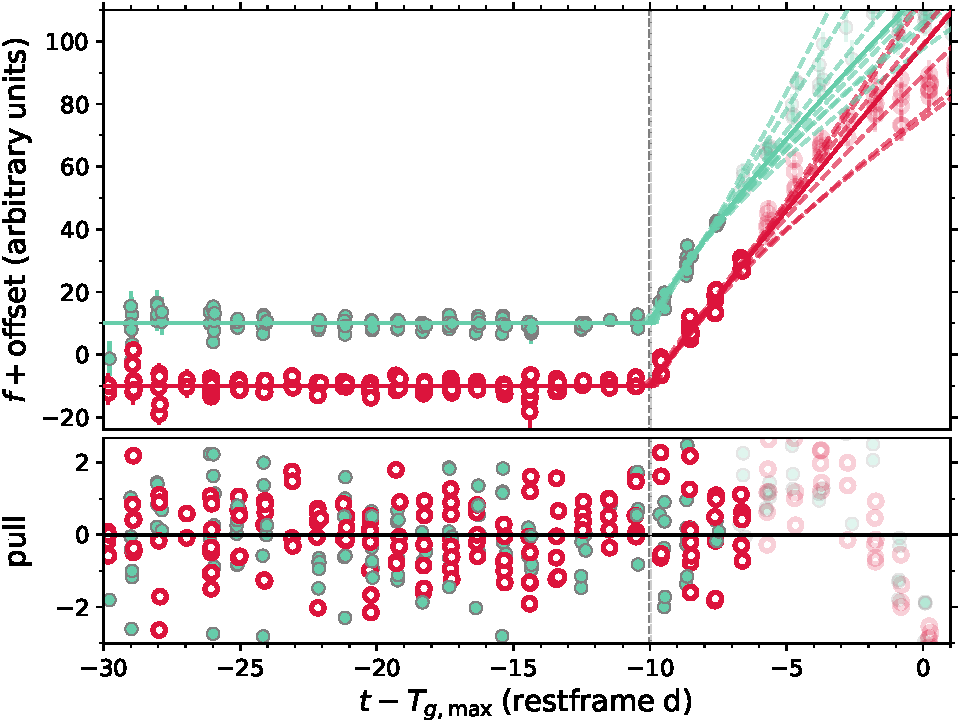
\includegraphics[width=3.4in]{./figures/ZTF18abclfee_model_lc.pdf}
    %
    \caption{Same as Figure~\ref{fig:corner_LC} for ZTF18abclfee, an 02cx-like
    SN with strong constraints on \tfl, and a short rise time. ZTF18abclfee has
    the tightest constraints on \trise\ of all 02cx-like SNe observed to date.}
    %
    \label{fig:02cx}
\end{figure}

ZTF18aaykjei (SN\,2018crl) is a Ia-CSM SN, with a long rise time. \trise$ = 22.8
\pm^{2.0}_{1.8}$\,d and $26.3 \pm 1$\,d for the uninformative and $\alpha = 2$
priors, respectively, which is significantly longer than the rise times of
normal SNe in this study. \citet{Silverman13} points out that Ia-CSM have
exceptionally long rise times, and \citet{Firth15} measure \trise$ > 30$\,d for
two of the SNe in the \citeauthor{Silverman13} sample. We also note that the
\rztf\ peak of ZTF18aaykjei occurs at least one week after the \gztf\ peak, as
has been seen in other Ia-CSM SNe \citep{aldering05gj,prieto05gj}.

There are two SC SNe Ia (ZTF18abdpvnd/SN\,2018dvf and ZTF18abhpgje/SN\,2018eul)
and two candidate SC SNe (ZTF18aawpcel/SN\,2018cir and ZTF18abddmrf/SN\,2018dsx)
identified in \citet{Yao19}. Each of these events exhibits a long rise, $\gtrsim
20$\,d and $\gtrsim 25$\,d for the uninformative and $\alpha=2$ priors,
respectively, as previously seen in other SC events (e.g.,
\citealt{Scalzo10,Silverman11}). We note that with the exception of
ZTF18abdpvnd, these events are detected at high redshift ($z \approx 0.15$), and
as a result the constraints on the individual rise time measurements are
relatively weak.

Finally, for ZTF18abdmgab, the 86G-like SN identified in \citet{Yao19}, we
cannot place strong constraints on the rise time due to a significant gap in the
observations around \tfl.

\section{Discussion}

\subsection{SNe Ia Rise Times}

In the analysis above, we provide multiple measurements of the rise time of SNe
Ia following the adoption of different priors. Within the literature, there are
at least a half dozen entirely different methods that have been employed to
answer precisely the same question. This naturally raises the question -- which
method is best? Which raises an important offshoot as well -- is the method
cheap to implement (i.e., does it provide reliable inference in the limit of
poor sampling or low SNR)?

\subsubsection{\texttt{SALT2} $X_1$ as a Proxy for \trise}

The ideal method to derive the rise time of SNe Ia would only use observations
obtained around maximum light, as these are relatively cheap to obtain and they
maximize the sample size for a flux-limited survey.
Figure~\ref{fig:tsquared_z_evolution} suggests that such a procedure may be
possible as there is a relatively tight linear relation between the
\texttt{SALT2} $X_1$ parameter and \trise\ (measured using the $\alpha = 2$
prior). Even in the limit of only one or a few observations on the rise,
\texttt{SALT2} can still measure $X_1$ (e.g., \citealt{Scolnic18a}). Thus, this
represents a far ``cheaper'' method for estimating the rise time than the
methods described above, which require high-cadence observations and the early
detection of a SN Ia.

For the volume-limited sample (see \S\ref{sec:volume_limited}) of normal SNe Ia
with known host galaxy redshifts and reliable model parameters, we estimate the
relation between \trise\ and $X_1$ via a maximum-likelihood linear-fit that
accounts for the uncertainties on both \trise\ and $X_1$ (see \citealt{Hogg10}).
From this fit we find
%
\begin{equation}
    t_\mathrm{rise} = (20.94 \pm 0.03) + (1.47 \pm 0.03)X_1\,\mathrm{d}.
    \label{eqn:rise_x1}
\end{equation} 
%
The residual scatter about this relation, as estimated by the sample standard
deviation, is 0.77\,d. We find the relation does not significantly change when
including SNe with unknown host-galaxy redshifts or unreliable model parameters
(though the scatter increases to $\sim$1.1\,d when including $z \ge 0.06$ SNe in
the fit). Thus, if one assumes $\alpha = 2$, then \texttt{SALT2} can be used to
estimate \trise\ with a typical uncertainty of $\sim$0.8\,d. This estimate is
only slightly worse than the median uncertainty on \trise, $\sim$0.5\,d, for the
$\alpha = 2$ prior. Furthermore, given that a $X_1 = 0$ SN is supposed to
represent a ``mean'' SN Ia, Equation~\ref{eqn:rise_x1} suggests that the mean
rise time of SNe Ia is $\sim$21\,d.

If we repeat the same exercise using uninformative prior rise times for the
volume limited sample, we find that the typical scatter about the linear
\trise-$X_1$ relation is $\sim$1.7\,d and $\sim$1.4\,d for the full and reliable
subsets of this sample. The mean rise time according to this relation is
$\sim$18\,d, however, we caution that this scatter is likely too large and mean
rise time too short, due to the systematic discussed in
\S\ref{sec:redshift_correlations}.

\subsubsection{Precise Estimates of \trise\ From Early Observations}

While the \trise-$X_1$ relation provides a relatively cheap method to infer the
rise time of normal SNe Ia, a significant advantage of early observations is
that they can provide far more precise estimates of \trise, especially in the
limit of low-redshift/high SNR. For the $\alpha = 2$ prior there are 14 SNe with
a half 68\% credible region that is $< 3$\,hr. For the uninformative prior this
number drops to two SNe. In either case, these measurements provide far more
precision than possible from \texttt{SALT2}.

While the methods adopted in this paper provide higher precision, it is
impossible that they are both accurate. The median difference in the inferred
\trise\ from the $\alpha = 2$ and uninformative priors for individual SNe is
4.7\,d. Even for the volume-limited subset of SNe with reliable model parameters
from the uninformative prior (15 total SNe) have a median difference in \trise\
estimates of 2.8\,d for the two priors. The systematic effect identified in
\S\ref{sec:redshift_correlations} suggests that the uninformative prior does not
provide accurate estimates of \trise, particularly for higher-$z$ SNe. The
$\alpha = 2$ prior, on the other hand, explicitly assumes that there is no
change in the early optical colors of SNe Ia. There is a large volume of
observations to disprove this particular assumption, raising the possibility
that neither method is accurate.

Empirical evidence suggests that $\alpha = 2$ prior is likely more accurate than
the uninformative prior (though again we caution that these estimates may still
be inaccurate). A SN cannot be detected until it has exploded, and thus the
epoch of discovery provides a lower limit on \trise. Between PTF/iPTF
\citep{Papadogiannakis19} and ZTF \citep{Yao19}, there are $\sim$20 SNe Ia that
are detected at least 18\,d prior to \tbmax, with a few detections as early as
18\,d prior to \tbmax. If the uninformative prior is accurate, then each of
these SNe would represent an incredibly lucky set of circumstances: (i) they
each have longer rise times than average, and (ii) they were all discovered
extremely soon after \tfl. A more probable explanation is that the mean rise
time is $> 18$\,d, in which case the $\alpha = 2$ prior provides a more accurate
inference of the rise time. The fact that each of the 4 SNe with $z < 0.03$,
which should have the least biased rise time estimates (see
\S\ref{sec:redshift_correlations}), have \trise$ > 18$\,d, further supports this
claim.

\subsubsection{Comparison to the Literature}

Several studies in the literature have attempted to measure the mean rise time
of SNe Ia. Here we compare our work to previous results. This exercise is
somewhat fraught with difficulty, in the sense that each study incorporates
slight differences in implementation, which, in turn, makes comparisons
challenging. Furthermore, these studies are typically conducted with different
filter sets and over a wide range of redshifts, which may introduce difficult to
understand biases across studies (as discussed above $K$-corrections are highly
uncertain at very early epochs). Finally, the quality of the data in each of
studies is vastyly different. For example, in the classic study by
\citet{Riess99a} there are a total of 7 observations spread across all the SNe
in their sample obtained more than 15\,d prior to \tbmax, while in contrast this
study includes 31 SNe \textit{discovered $> 15$\,d before \tbmax} \citep{Yao19}.
As we proceed with our cross-study comparison, we exclude rise time estimates
for individual SNe and instead focus on studies with relatively large samples
($\gtrsim 10$ normal SNe Ia).

As previously outlined, there are broadly two different methods to measure the
mean rise time of SNe Ia. The first uses ``shape-corrected'' light curves,
whereby all individual light curves are stretched by some empirically measured
factor, and the mean rise time represents a normal SN Ia after shape correction
(e.g., \citep{Riess99a,Conley06,Hayden10,Ganeshalingam11}). The second method is
to measure the rise time of every individual SNe Ia within a sample, and then
take the mean of this distribution. These two methods are not equivalent, and
therefore are likely to produce different results. If, for instance, nature
produces more high-luminosity, slower-declining SNe Ia than low-luminosity,
faster-declining events, then the population mean will produce longer rise times
shape-corrected mean, as this latter method normalizes all the light curves to
be the same. Even if nature is not biased, flux-limited surveys, such as ZTF,
will always find more slower-declining SNe than fast decliners, leading to
potentially longer rise time estimates for the population mean relative to a
stretch-corrected estimate.

Using different data sets obtained in very different redshift regimes,
\citet{Riess99a} and \citet{Conley06} estimate consistent values of the
shape-corrected mean \trise$ \approx 19.5$\,d. Each of these studies fixes
$\alpha = 2$ when fitting for the rise time. This estimate is roughly half way
inbetween our estimates of the mean rise time from the uninformative prior and
the $\alpha = 2$ prior. As noted above, these two measurements are not the same,
which likely explains their difference. Later studies by \citet{Hayden10} and
\citet{Ganeshalingam11}, also provide estimates of the mean shape-corrected rise
time and find smaller values of $\sim$17.5--18.0\,d. As noted by
\citeauthor{Hayden10}, these methods are highly dependent on the template light
curve used to stretch the individual SNe, and differences in the templates
between these studies may explain the dissensus between these studies.


The approach employed in \citet{Zheng17a}, \citet{Papadogiannakis19}, and
\citet{Firth15} is more similar to the one adopted here, as each of these
studies estimates the rise time for many individual SNe and then calculates the
population mean. If the samples differ between any of these studies, and aside
from 11 SNe that are included in both \citet{Papadogiannakis19} and
\citet{Firth15} there is no overlap between any of studies or this one, then it
should be expected that the population mean rise time estimates will differ.
Furthermore, the \trise\ estimates in \citet{Papadogiannakis19} and
\citet{Firth15} are not relative to \tbmax, and it is known that the rise time
increases as one progressively moves to redder wavelengths (e.g.,
\citealt{Ganeshalingam11}). Taken together, this confluence of factors makes it
difficult to compare results between these studies, which we nevertheless do
below.

In \citet{Zheng17}, a semi-analytical, six parameter, broken power-law model is
introduced to describe the optical evolution of SN Ia. This model has a distinct
advantage over the methods employed here in that an artificial cutoff does not
need to be applied in flux-space (see \S\ref{sec:model}), though a post-peak cut
must be applied as the model cannot reproduce the evolution of SNe into the
nebular phase. A downside of this approach is that there are large degeneracies
between the different model parameters, meaning it is difficult to find
numerically stable solutions without fixing individual parameters to a single
value \citep{Zheng17a}. For a sample of 56 well-observed low-$z$ SNe this method
produces a mean rise time of 16.0\,d \citep{Zheng17a}, while the same technique
applied to SNe Ia from PTF/iPTF finds a mean rise time of 16.8\,d
\citep{Papadogiannakis19}. These estimates are considerably lower than the ones
presented here, and are almost certainly underestimates of the true mean rise
time based on the large number of SNe with detections $>$16\,d before peak
\citep{Papadogiannakis19, Yao19}. Indeed, close inspection of Figure~1 in
\citet{Zheng17a} shows that the six-parameter model underestimates the flux at
the very earliest epochs and underestimates \trise\ as a result.

The closest comparison to the methods used in this study can be drawn from
\citet{Firth15}. Using a sample of 18 SNe discovered by PTF and the La Silla
Quest (LSQ) survey, \citeauthor{Firth15} fit a model similar to
Equation~\ref{eqn:flux_model}, in that \tfl\ and $\alpha$ are allowed to
simultaneously vary. From these fits, they estimate a mean population \trise$ =
18.98 \pm 0.54$\,d, which is consistent with our estimate of the rise time for
the volume-complete $z_\mathrm{host}$ sample, $\sim$18.5\,d. Contrary to this
study, they find shorter rise times, and a mean of $\sim$17.9\,d, when fixing
$\alpha = 2$ (this is likely explained by their adopted fit procedure, see
below). As explained in \S\ref{sec:redshift_correlations}, the \trise\ estimates
in \citet{Firth15} are likely underestimated due to the bias introduced for
models with uninformative priors.

\subsection{The Expanding Fireball Model}

The expanding fireball model (see \S\ref{sec:model}) is remarkable in its
simplicity. The two underlying assumptions of the expanding fireball model, that
the photospheric velocity and temperature of the ejecta are $\sim$constant
during the early evolution of the SN, are clearly over-simplifications
(\citealt{Parrent12} shows that the photospheric velocity declines by at least
33\% in the $\sim$5\,d after explosion). This makes it all the more remarkable
that numerous studies have found that $\alpha$ is consistent with 2, as
predicted by the fireball model (e.g.,
\citealt{Conley06,Hayden10,Ganeshalingam11,Gonzalez-Gaitan12,Zheng17a}).

Indeed, we find the same in this study, $\alpha_r = 2.01 \pm 0.03$ (for the
volume-limited subset of normal SNe Ia with reliable model parameters). We
separately find $\alpha_g > 2$, which is sensible given that $\alpha_g =
\alpha_r = 2$ implies no color change. Furthermore, following the arguments of
\citet{Riess99a}, \rztf\ features less line absorption and is farther into the
Rayleigh-Jeans tail, making it reasonable that the assumptions hold better there
than in the \gztf\ filter.

At the same time, there are individual SNe for which the expanding fireball
model simply does not apply. This has been clearly shown for SN\,2013dy and
iPTF\,16abc \citep{Zheng13,Miller18}, and within this study that is clearly the
case for ZTF18aasdted (SN\,2018big), the lowest redshift SN in our sample, where
the DIC clearly prefers $\alpha \approx 1.5$ to $\alpha = 2$. A reasonable
conclusion, therefore, is that for SNe Ia $\alpha = 2$ provides an acceptible
proxy for the early evolution of most SNe Ia. It also stands to reason that
individual SNe exhibiting significant departures from $\alpha = 2$ are not
typical, and they may be the result of exotic explosion or companion scenarios
(see also \citealt{Miller18}). Moving forward, it may be that the most
appropriate prior for fitting the early evolution of SNe Ia is to adopt a
Gaussian centered at 2 for $\alpha$ in the redder filters, while also placing a
prior on the difference in $\alpha$ across different filters (for ZTF $\alpha_r
- \alpha_g \approx -0.17$ based on \S\ref{sec:colors}). More observations,
especially of low-$z$ SNe, and testing, are needed to confirm whether or not
such priors are in fact appropriate.

Finally, we note that the analysis in \citet{Firth15} stands in contrast to this
study, and those listed above, in that the mean value of $\alpha = 2.44 \pm
0.13$, which is not consistent with 2. This result can be understood in the
context of the \citet{Firth15} fitting procedure, whereby an initial estimate of
\tfl\ is made by fixing $\alpha = 2$. Only obversations obtained 2 days before
and after this initial \tfl\ estimate are included in the final model fit (i.e.,
the entire baseline of non-detections is not used, as is done in this study).
Truncating the baseline biases the model to longer rise times (as is observed in
\citealt{Firth15}), and, as shown in Figure~\ref{fig:corner_LC}, longer rise
times require larger values of $\alpha$ when adopting the model used in this
study and \citep{Firth15}.

\section{Conclusions}

In this paper we have presented an analysis of the initial evolution and rise
times of 127 ZTF-discovered SNe Ia with early observations (see \citealt{Yao19}
for details on how the sample was selected). These SNe were observed as part of
the ZTF high-cadence extragalactic experiment, which obtained 3 \gztf\ and 3
\rztf\ observations every night the telescope was open. A key distinction of
this data set relative to many previous studies is the large number of
observations taken prior to the epoch of discovery, which meaningfully
constrains the behavior of the SN at very early times. The uniformity, size and
observational duty cycle of this data set are truly unique, making this sample
of ZTF SNe the premiere data set for studying the early evolution of
thermonuclear SNe.

We model the early evolution of these SNe as a power-law in time $t$, whereby
the flux $f \propto (t - t_\mathrm{fl})^\alpha$, where \tfl\ is the time of
first light, and $\alpha$ is the power-law index. By simultaneously fitting
observations in the \gztf\ and \rztf\ filters, we are able to place stronger
constraints on \tfl\ than would be possible with observations in a single
filter. While many previous studies have fixed $\alpha = 2$, following the
simple expanding fireball model (e.g., \citealt{Riess99a}), we have instead
allowed $\alpha$ to vary, as there are recent examples of SNe Ia where $\alpha$
clearly does not equal 2 (e.g., \citealt{Zheng13, Miller18,Shappee16}). While
the population mean value of $\alpha$ tends towards 2, there are several SNe for
which it is clear that $\alpha \ne 2$, justifying our model parameterization.

As might be expected, we find that our ability to constrain the model parameters
is highly dependent on the quality of the data. Lower redshift, and hence higher
SNR, SNe without significant gaps in observational coverage are better
constrained than their high-redshift counterparts or events will large temporal
gaps. We identify those SNe with reliable model parameters under the reasonable
assumption that models of the initial flux evolution should over-estimate the
flux at peak brightness. Following this procedure we find that 51 of the SNe
have reliable model parameters. We focus our analysis on these events.

For the subset of normal SNe with reliable model parameters we estimate a
population mean \trise$ \approx 18.0$\,d, with a sample standard deviation of
$\sim$1.6\,d about this mean. For individual SNe, the range of rise times in our
data set extends from $\sim$14--22\,d. We have additionally identified a
systematic in the parameter estimation for models that simultaneously vary \tfl\
and $\alpha$. Namely, for flux limited surveys, the model constraints on \trise\
will be biased and underestimated for the higher redshift SNe in the sample. If
we restrict the sample to a volume-limited subset of SNe ($z < 0.06$), where
this bias may still be present, but it should be less prevalent, we estimate a
mean population rise time of $\sim$18.5\,d.

Normal SNe Ia have a population mean $\alpha_g \approx 2.1$ and a population
mean $\alpha_r \approx 2.0$, with a population standard deviation $\sim$0.5 for
both parameters. While the mean value for our sample of SNe tends towards 2, as
would be expected in the expanding fireball model, we observe a range in
$\alpha$ extending from $\sim$1.0--3.5. For both \trise\ and $\alpha$, there is
no single value that is consistent with all the SNe in our sample.
Interestingly, however, we do find that nearly all SNe are consistent with a
single value of $\alpha_r - \alpha_g$, which describes the initial \gztf$ -
$\rztf\ color evolution of SNe Ia. The data show a mean value of $\alpha_r -
\alpha_g \approx -0.17$, meaning the optical colors of most SNe Ia evolve to the
blue with comparable magnitudes over a similar timescale. This could be a sign
that the degree of $^{56}$Ni-mixing in the SN ejecta is very similar for the
majority of SNe Ia (e.g., \citealt{Piro16}).

We find that the rise time is correlated with the SN shape, in the sense that
high-luminosity, slowly-declining SNe have longer rise times. This is true
whether the shape is parameterized by the \texttt{SALT2} $X_1$ parameter, or the
decline in the \gztf\ band in the 15\,d after peak brightness, $\Delta
m_{15}(g_\mathrm{ZTF})$. This finding is consistent with many previous studies.

Given the large number of SNe with unreliable model parameters, and the observed
bias in the measurement of \trise\ for high-$z$ SNe, we also consider how the
model parameter estimates change with strong priors. In particular, we adopt
$\alpha_g = \alpha_r = 2$, enforcing the expanding fireball hypothesis on the
data. Strictly speaking, this prior means that the early colors of SNe Ia do not
change, which we empirically know is not the case (see above). Nevertheless, a
$\sim$constant temperature is one of the assumptions of the fireball model, and,
thus we proceed.

Under the $\alpha = 2$ prior, we find that far more SNe have reliable \trise\
estimates. For the typical SN in our sample, fixing $\alpha = 2$ results in an
increase in \trise\ by a few days. We estimate a population mean \trise$ \approx
21.0$\,d when adopting the $\alpha = 2$ prior. One consequence of adopting this
prior is that it significantly reduces the previously observed bias where
high-$z$ SNe are inferred to have shorter rise times. The use of this prior also
reduces the scatter in the $X_1$--\trise\ relation, and we find that with
\texttt{SALT2}, via the measurement of $X_1$, it is possible to estimate \trise\
with a typical scatter of $\sim$0.77\,d, even if there are no early time
observations available. We also find that, for the vast majority of the SNe in
our sample, all but 13 events, there is only weak evidence that the $\alpha \ne
2$ model is preferred to a model with $\alpha_g = \alpha_r = 2$ according to the
DIC.

While we have primarily focused on the properties and evoltion of normal SNe Ia,
there are 7 SNe in our sample that cannot be catagorized as normal (see
\citealt{Yao19}). As in previous studies, we find that the rise times of Ia-CSM
SNe and SC explosions are longer than those of normal SNe Ia. We highlight our
observations of ZTF18abclfee, an 02cx-like with exquisite observational coverage
in the time before explosion. We estimate the \tfl\ to within $\sim$8\,hr for
ZTF18abclfee, making our measurement the most precise estimate of \trise\ for
any 02cx-like SN to date. ZTF18abclfee took $\sim$10\,d to reach peak
brightness, roughly 5\,d less than SN\,2005hk, another 02cx-like event with a
well-constrained rise time.

This study has important lessons for future efforts to characterize the rise
times of SNe Ia. We have found that for all but the best-observed, low-$z$
events, a generic power-law model where $\alpha$ is allowed to vary does not
place meaningful constraints on the \trise, or worse, in the case of high-$z$
events, it produces a biased estimate. If this were the end of the story, it
would be particularly bad news for the Large Synoptic Survey Telescope (LSST),
which will typically have several day gaps in its observational cadence
\citep{Ivezic08}. With only Equation~\ref{eqn:flux_model} at our disposal, we
would rarely be able to infer \trise\ for LSST SNe. We have also shown, however,
that in the limit of lower-quality data, meaning low SNR or infrequent cadence,
the application of a prior to the model can significantly improve the final
inference (for example, the significant reduction in the $X_1$--\trise\ relation
after adopting an $\alpha = 2$ prior). The challenge, at the moment, is
developing an empirically supported prior for the model parameters. This
provides a strong justification for the concurrent operation of LSST and
small-aperture, high-cadence experiments, such as ZTF and the planned ZTF-II.
These smaller, more focused, missions can provide exquisite observations of a
select handful of SNe that can be used to drive the priors in our inference.
While there have been thousands of SNe Ia studied to date (e.g.,
\citealt{Jones17}), indeed more examples are still needed: there are only 4
normal, $z < 0.03$ SNe Ia in our sample, and these 4 are nearly as valuable as
the remainder of the sample for established the diversity of SNe Ia. As we
improve our understanding of these priors, and combine that knowledge with the
hitherto unimaginable statistical samples from LSST ($\sim$millions of SNe), we
will definitively understand the early evolution and distribution of rise times
for Type Ia SNe.


\acknowledgements

Dan F-M? Will Farr?

\software{
         % \texttt{astropy} \citep{Astropy-Collaboration13},
          \texttt{scipy} \citep{Jones01}, 
          \texttt{matplotlib} \citep{Hunter07},
          \texttt{pandas} \citep{McKinney10},
          \texttt{emcee} \citep{Foreman-Mackey13},
          \texttt{corner} \citep{Foreman-Mackey16},
          \texttt{SALT2} \citep{Guy07}
          }

%% For this sample we use BibTeX plus aasjournals.bst to generate the
%% the bibliography. The sample63.bib file was populated from ADS. To
%% get the citations to show in the compiled file do the following:
%%
%% pdflatex sample63.tex
%% bibtext sample63
%% pdflatex sample63.tex
%% pdflatex sample63.tex

\appendix

\section{Quality Assurance}\label{sec:qa}

As noted in \S\ref{sec:model}, the MCMC model converges for all but one ZTF
SNe within the sample. However, visual inspection of both the corner plots and
individual draws from the posterior quickly reveals that for some SNe the data
do not provide strong constraints on the model parameters (see the bottom row
of Figure~\ref{fig:corner_LC}). In the most extreme cases, as shown in
Figure~\ref{fig:biggap_lc}, large gaps in the observations make it nearly
impossible to constrain the model parameters. For these cases, the model
posteriors are essentially identical to the priors (there is always a weak
constraint on \tfl\ from epochs where the SN is not detected).

\begin{figure}
    \centering
    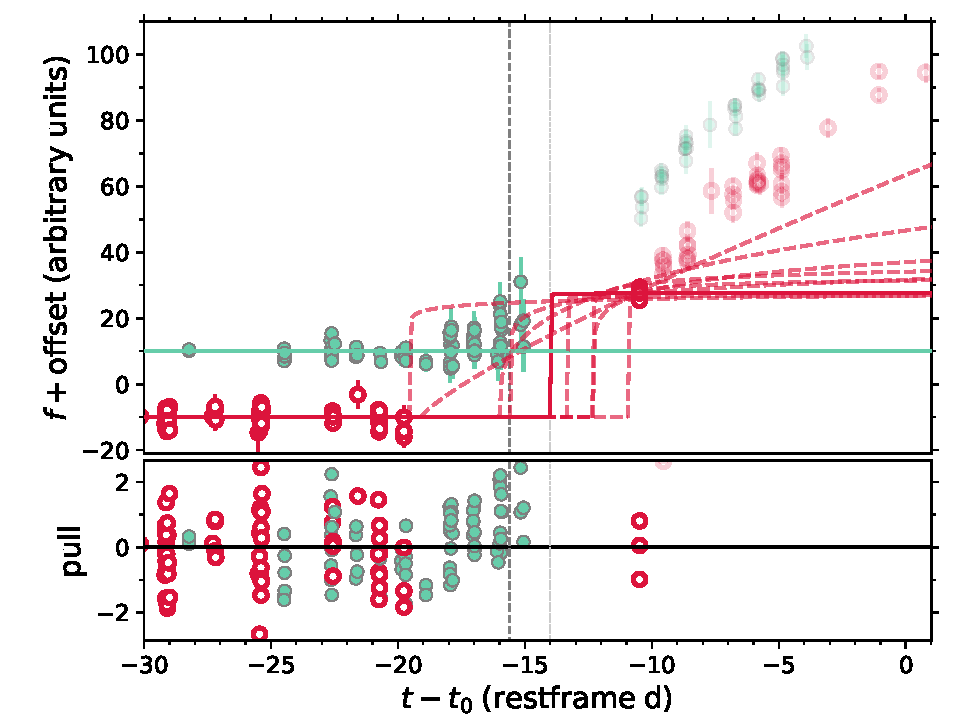
\includegraphics[width=3.4in]{./figures/ZTF18aaqffyp_model_lc.pdf}
    %
    \caption{Same as Figure~\ref{fig:corner_LC} for ZTF18aaqffyp, a SN with
    observations that place very weak constraints on \tfl. The marginalized
    posteriors for $A^\prime$ and $\alpha$ are essentially identical to the
    priors. Posteriors with little information beyond the prior are typical
    of SNe with significant observational gaps.}
    %
    \label{fig:biggap_lc}
\end{figure}

To identify SNe with poor observational coverage, or unusual structure in the
posterior, we visually examine the light curves and corner plots for each of
the 127 SNe in our sample. We flag SNe where the model significantly
underestimates the flux near \tbmax\ (similar to what is shown in
Figure~\ref{fig:biggap_lc}), as this is a good indicator that the model has
poor predictive value. By definition the light curve derivative is zero at
maximum light, and the relative change in brightness constantly slows down in
the $\sim$week leading up to maximum light. Therefore, models of the early
emission should greatly over-predict the flux at maximum, which is why we
adopt this criterion for flagging SNe with poorly constrained model
parameters.

Numerically, the visually flagged SNe can, for the most part, be identified
by a combination of two criteria: the 90\% credible region on \tfl,
$\mathrm{CR}_{90}$, and the number of nights on which the SN was detected.
Rather than providing a threshold for detection (e.g., $3\sigma$, $5\sigma$,
etc.), we count all nights with $f_\mathrm{mean} \le 0.4 f_\mathrm{max}$
after the median marginalized posterior value of \tfl\ with observations in
either the \gztf, \rztf, or both filters, $N_{g, \mathrm{det}}$, $N_{r,
\mathrm{det}}$, and $N_{gr, \mathrm{det}}$, respectively. We take the
geometric mean of these three numbers to derive the ``average'' number of
nights on which the SN was detected, $\mathrm{GM}(N_\mathrm{det})$. A scatter
plot showing $\mathrm{GM}(N_\mathrm{det})$ vs.\ $\mathrm{CR}_{90}$ is shown
in Figure~\ref{fig:flagged_sn}. Visually flagged SNe are shown as orange
circles, while $+$ symbols show those that were not flagged.

\begin{figure*}
    \centering
    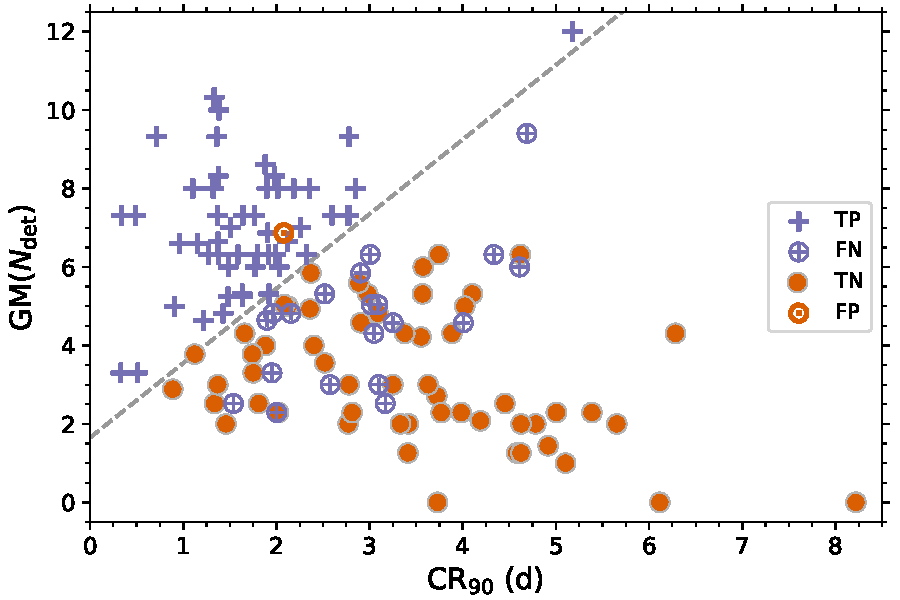
\includegraphics[width=5in]{./figures/final_sample.pdf}
    %
    \caption{Scatter plot showing the distribution of the 127 ZTF SNe Ia in
    the $\mathrm{GM}(N_\mathrm{det})$--$\mathrm{CR}_{90}$ plane. Models with
    flagged posterior parameters are shown as orange circles, while those
    that are not flagged are shown via $+$ symbols. The dashed line shows the
    adopted separation threshold for identifying reliable model fits (above
    the line), and unreliable model fits. FP and FN (see text) SNe are
    circled. }
    %
    \label{fig:flagged_sn}
\end{figure*}

The visual inspection procedure described above is not fully reproducible
(visual inspection is by its very nature subjective). Therefore, we aim to
separate the SNe into two classes (reliable and unreliable) via an automated,
systematic procedure. Treating the visually flagged sources as the negative
class, we view false positives (i.e., visually flagged SNe that are included
in the final population analysis) particularly harmful. Therefore, we adopt
%
$$ \mathrm{GM}(N_\mathrm{det}) \ge 1.9\,\mathrm{CR}_{90} + 1.65,$$
%
as the classification threshold for reliable model fits (as shown via the
dashed line in Figure~\ref{fig:flagged_sn}). This threshold retains 50 true
positives (TP; visually good models included in the final sample) with only a
single false positive (FP; visually flagged SNe in the final sample). This
choice does result in 20 false negatives (FN; visually good models
\textit{excluded} from the final sample), while all remaining flagged SNe are
true negatives (TN). Further scrutiny of the FN reveals several light curves
with significant observational gaps, which, as discussed above, makes it
difficult to place strong constraints on the model parameters. Ultimately,
our two-step procedure identifies 51 SNe as reliable, while 76 are excluded
from the final population analysis due to their unreliable constraints on the
model parameters.

\section{Systematics}\label{sec:systematics}


\bibliography{/Users/adamamiller/Documents/tex_stuff/papers}
\bibliographystyle{aasjournal}

%% This command is needed to show the entire author+affiliation list when
%% the collaboration and author truncation commands are used.  It has to
%% go at the end of the manuscript.
%\allauthors

%% Include this line if you are using the \added, \replaced, \deleted
%% commands to see a summary list of all changes at the end of the article.
%\listofchanges

\end{document}

% End of file `sample63.tex'.
